\documentclass[UTF8,a4paper,11pt,fontset=fandol]{ctexart}
\IfFontExistsTF{Droid Sans Fallback}
  {\newCJKfontfamily\cjkfallback{Droid Sans Fallback}}
  {\IfFontExistsTF{Noto Sans CJK SC}
    {\newCJKfontfamily\cjkfallback{Noto Sans CJK SC}}
    {\newcommand{\cjkfallback}{\CJKfamily{song}}}}
\usepackage[margin=22mm,headheight=15pt]{geometry}
\usepackage{graphicx,float,xcolor,amsmath,amssymb,booktabs,longtable,array,tabularx}
\usepackage[most]{tcolorbox}
\usepackage{listings,needspace,fancyhdr,enumitem}
\setlist{leftmargin=2em,itemsep=0.35em,topsep=0.4em,parsep=0pt}
\usepackage[unicode,colorlinks=true,linkcolor=blue!45!black,urlcolor=blue!45!black,breaklinks=true]{hyperref}
\usepackage{xurl}
\setlength{\parindent}{0pt}
\setlength{\parskip}{0.65em}
\setlength{\emergencystretch}{3em}
\linespread{1.14}
\raggedbottom
\pagestyle{fancy}\fancyhf{}\fancyhead[L]{月球大叔 · 访谈学习笔记}\fancyfoot[C]{\thepage}
\newtcolorbox{importantbox}[1]{enhanced,breakable,colback=blue!3,colframe=blue!45!black,title={#1},fonttitle=\bfseries}
\newtcolorbox{knowledgebox}[1]{enhanced,breakable,colback=teal!3,colframe=teal!50!black,title={#1},fonttitle=\bfseries}
\newtcolorbox{warningbox}[1]{enhanced,breakable,colback=orange!4,colframe=orange!60!black,title={#1},fonttitle=\bfseries}
\lstset{basicstyle=\ttfamily\small,breaklines=true,columns=fullflexible,keepspaces=true,showstringspaces=false,frame=single,captionpos=b}
\newcolumntype{Y}{>{\raggedright\arraybackslash}X}
\newcommand{\notetitle}{AI 算力怎样变便宜：肖志斌谈芯片、推理与系统优化}
\newcommand{\videocoverpath}{cover.jpg}
\newcommand{\videourl}{https://www.youtube.com/watch?v=gxeP0tAm8mc}
\newcommand{\videochannel}{月球大叔}
\newcommand{\videopublishdate}{2026-09-07}
\newcommand{\noteauthors}{月球大叔、肖志斌}
\newcommand{\sourceurl}{https://www.youtube.com/watch?v=gxeP0tAm8mc}
\begin{document}

\begin{titlepage}\centering\vspace*{4mm}
{\Large 月球大叔 · EP06 访谈学习笔记\par}\vspace{8mm}
{\LARGE\bfseries \notetitle\par}\vspace{7mm}
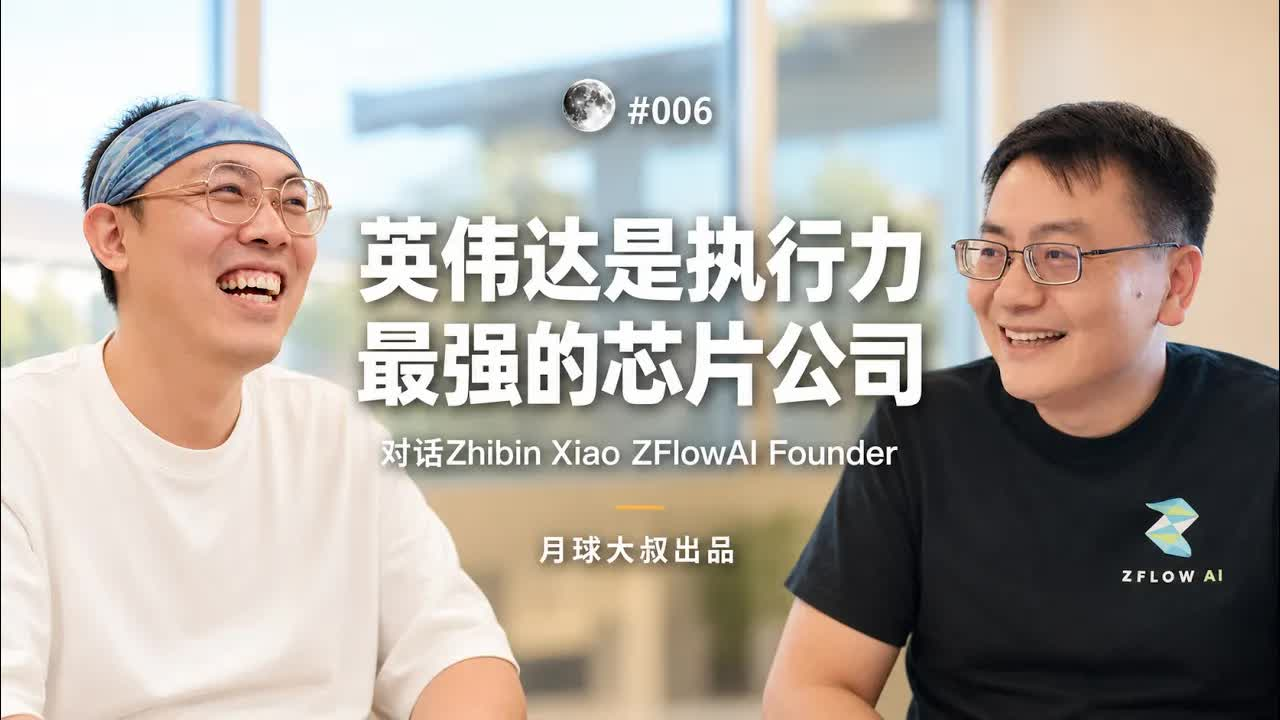
\includegraphics[width=.86\linewidth,height=.27\textheight,keepaspectratio]{cover.jpg}
\par\vspace{6mm}{\small 原节目：肖志斌：AI芯片，英伟达，全球供应链，2纳米，中美日韩，Groq，Cerebras，SambaNova，创业，AI原生\par}
\vspace{4mm}主播：月球大叔\par
{\small 嘉宾：肖志斌\par}
\vfill 发布：2026-09-07\par
整理：2026-10-25\quad 正文：Gemini Argon\quad 配图与编校：Codex\par
\vspace{4mm}\url{https://www.youtube.com/watch?v=gxeP0tAm8mc}
\end{titlepage}
\begingroup\small\setlength{\parskip}{0pt}\tableofcontents\endgroup\clearpage
\section*{导读}\addcontentsline{toc}{section}{导读}
当大模型走向规模化应用，算力紧缺与词元（token）成本居高不下成为行业共同面对的现实问题。本书依据芯片架构师、ZFlow.AI 创始人肖志斌的深度访谈整理而成，从计算机体系结构与软硬件协同设计的视角，拆解“AI 算力怎样变便宜”这一核心命题。全书顺着肖志斌从浙江大学 MIPS/DSP 研发、UC Davis 众核数据流研究、Oracle SPARC 数据库加速芯片、阿里含光 800 到系统优化创业的技术脉络，依次剖析芯片从需求定义到量产的工业链条、全球半导体供应链与先进制程的物理机制、大模型预填充（prefill）与解码（decode）阶段的算力及内存瓶颈、非传统数据流架构与英伟达的系统壁垒，以及如何借助经实机校准的虚拟仿真探索更经济的软硬件配置。
\needspace{8\baselineskip}\section{从造芯片到优化系统：算力问题的边界}
作为全书的开篇，本章通过芯片架构师肖志斌二十余年的技术演进路径，回答一个核心问题：当半导体制造工艺逼近物理放缓期时，人工智能算力的竞争主战场为何从单颗芯片的晶体管堆叠，转向软硬件协同与系统级优化？我们将梳理处理器架构从音视频编解码、众核数据流、数据库硬件加速到 AI 系统的演进脉络，明确有效算力的技术边界。
\needspace{6\baselineskip}\subsection{从浙大到 UC Davis、Oracle 与阿里}
1999 年，肖志斌考入浙江大学竺可桢学院，本科修读电子工程（EE）。促使他转向芯片与架构设计的契机，是本科阶段修读的计算机组成与计算机体系结构课程。当时，发明 CPU 分支预测（branch prediction）架构的得州大学奥斯汀分校（UT Austin）教授 Yale Patt 到浙大暑期授课，这门课让肖志斌确立了对计算机体系结构（computer architecture）的长期兴趣。嘉宾回顾，自己过去二十多年的工作始终围绕软硬件协同设计与架构设计展开，核心目标一直是让系统更高效地完成计算（00:01:43）。

2002 至 2003 年间，他在浙大从本科到研究生阶段参与了类似 863 计划的自主 CPU 与数字信号处理器（DSP）正向研发项目。研究生的具体课题是在传统 MIPS 指令集架构处理器上做多媒体指令扩展，设计单核 DSP 来处理 VCD 时代的 MPEG 语音与视频编解码。随后他赴美在加州大学戴维斯分校（UC Davis）攻读博士，研究方向从单核演进为众核（Manycore）DSP，核心是采用数据流计算（dataflow computing）做流式处理，用于解决通信、视频编解码以及大数据查询与排序问题。

在博士阶段的众核架构中，每个 DSP 核心（core）的指令与数据存储器（memory）都很小，核心之间通过片上互连网络衔接，并可独立调节各自的频率和电压。这种让数据在众多核心之间直接流动、尽量减少向芯片外部读写的设计，与如今许多 AI 处理器的数据流架构十分相似。从早期的多媒体处理到片上数据流，再到后来的企业级系统与 AI 算力，肖志斌的技术演进经历了四个紧密衔接的阶段，每一个阶段的经历都服务于他对“系统瓶颈在哪里”这一问题的持续追问：
\begin{enumerate}
\item 单核指令扩展：在浙大基于 MIPS 扩展多媒体指令，实现 MPEG 音视频编解码。
\item 众核片上数据流：在 UC Davis 研究众核 DSP，让数据在片上核心间流动并支持独立调频调压。
\item 处理器内嵌数据库加速：在甲骨文（Oracle）参与将数据库算子硬化为 SPARC CPU 内部的协处理器。
\item 专用 AI 芯片与系统优化：在阿里巴巴研发第一代 AI 芯片含光 800，随后创业做稀疏化 AI 芯片，进而转向 AI 系统仿真与优化。
\end{enumerate}

博士毕业后，肖志斌加入此前收购了太阳微系统公司（Sun Microsystems）的 Oracle（口述中一度误作 2017 年，后文 01:10:01 与 01:24:09 明确其为 2012 年博士毕业进入 Oracle 工作五年至 2017 年）。当时服务器市场主要有 SPARC、IBM PowerPC 和 x86 三类大型指令集，SPARC 服务器配合 Solaris 操作系统以长年无需关机的高稳定性著称。为了结合 Oracle 的数据库主业做创新，团队在 SPARC 处理器内部设计了数据库加速单元（DAX，00:05:20）。他们针对包含 22 条查询（query）的 TPC-H 数据库性能基准测试（Benchmark），将核心算子硬化到硬件中，设计专用指令集与运行时系统（runtime），使其成为数据库查询优化器（query optimizer）的加速器。该协处理器与 CPU 共享全部内存带宽，能够用满（saturate）带宽以支持高速的内存型（in-memory）数据库处理。在 Oracle 工作五六年并于 2017 年离开后，他加入阿里巴巴研发第一代 AI 芯片含光 800，随后又参与创立了一家专注稀疏化 AI 芯片的公司。

\needspace{6\baselineskip}\subsection{为什么不再直接造一颗新芯片}
经历从 CPU 内嵌加速器、专用 AI 芯片到稀疏芯片的完整研发周期后，肖志斌在最新一次创业中选择了不再直接造芯片，而是创办系统优化公司 ZFlow.AI。主持人提问，这种转型是否意味着 AI 性能竞争的主战场正从晶体管转向软件与系统开发。肖志斌给出了肯定的回答：随着摩尔定律放缓，单芯片层面的算力提升与功耗降低正越来越成为瓶颈，真正的卡点已经转移到了系统层次和软件层次（00:08:10）。

从行业分工来看，目前市面上已经有大量创业公司和巨头在解决单颗 AI 芯片的设计问题。嘉宾强调，如果自己做的事情不再是行业最痛的瓶颈，架构师就应该转身去解决新的系统级瓶颈。在当下的 AI 基础设施中，异构系统软件、模型切分与集群通信的复杂度急剧上升，单纯依靠硬件堆料已无法经济地换取性能提升。

此外，大规模 AI 集群价格昂贵，许多系统工程师在日常开发中没有充足的真实物理硬件可供调优试错。针对这一痛点，ZFlow.AI 将模型编译、运行时调度以及 AI 系统仿真整合到一个统一平台中，结合仿真与自动性能分析（profile），让客户在没有拿到实体硬件、甚至硬件尚未制造出来之前，就能在虚拟环境中探索各种软硬件优化方案。

这一工具链最终要回答一个核心的经济学问题：究竟什么样的模型跑在什么样的硬件上是最经济的？这里的目标硬件既包括市面上已有的商业芯片，也涵盖尚未流片的未来架构。肖志斌同时保留了架构师的开放视野：系统仿真与优化实际上是所有芯片设计公司立项前必须完成的前置工作；如果在仿真推演中发现某类高价值负载特别契合某种新架构，团队也完全有可能顺势孵化出新的芯片项目。

\needspace{6\baselineskip}\subsection{芯片、软件与应用共同决定有效算力}
在探讨何时才值得真正造一颗专用芯片时，嘉宾指出这取决于上层应用与模型架构是否已经收敛（converge）。如果某个特定任务——例如扫地机器人，或者停车场内的车辆监测——其算法模型已经基本固化且能满足人类需求，不再频繁变动，那么针对该任务定制专用芯片就能获得明显的能效与成本优势。

节目讨论中提到了加拿大初创公司 Taalas 的案例。这家公司由另一家 AI 推理芯片公司 Tenstorrent（现由架构师 Jim Keller 担任 CEO）的创始人创立，其特点是尝试把特定模型直接固化在芯片里（00:11:50）。肖志斌解释，投资人之所以支持这种路线，是因为在特定任务下当模型趋于固化时，从经济效益上看值得将其硬化到芯片中；但这也意味着其适用前提是目标模型与任务相对稳定，若模型结构仍在快速变化，还需权衡适配成本与芯片产品周期。

关于其内部实现，肖志斌根据自己的理解解释说，Taalas 的架构并非完全不可调整，而是在芯片设计中保留了多层金属层（metal）的调整空间：当模型需要改动时，可以对其中几层金属层重新流片，即通过金属层修正（metal fix）来适配。按照嘉宾的解释，这种方式虽然仍涉及晶圆厂的制造加工环节、代价不同于纯软件更新，但相比每次重新制作全套掩膜（full mask）的完整流片，成本要低得多，相当于在制造层面保留了一定程度的定制灵活性。

由此可见，AI 时代的算力供给不是单一维度的硬件竞赛，而是由应用特征、软件栈与芯片架构共同决定的平衡：
\begin{enumerate}
\item 通用高灵活性路线：依靠通用处理器加软件栈，适应快速演进的大模型，但需承担数据搬运与调度的系统开销。
\item 金属层修改路线：如嘉宾讨论的 Taalas 方案，借助局部金属层修正，在模型相对收敛时兼顾专用电路能效与有限的模型调整能力，但仍受制于制造环节的周期与成本。
\item 专用硬件加速路线：当特定任务（如大规模视频流转码或固定场景监测）的算法流程稳定后，将核心算子硬化为专用芯片（其中仍可配合必要的控制与可编程模块），以降低总拥有成本（TCO）与功耗。
\end{enumerate}

\begin{importantbox}{片上数据流计算（Dataflow Computing）}
传统处理器计算时，往往需要频繁将数据从片外内存读入计算核心，算完后再写回片外，导致大量时间与功耗浪费在数据搬运和内存带宽等待上。肖志斌在博士阶段研究的众核 DSP 数据流架构，核心机制是让每个核心配备极小的本地存储，通过片上互连网络直接传递中间结果。数据像流水一样在芯片内部的众多核心之间连续流转并完成处理，尽量不流出芯片外部，这一思想也成为当今许多专用 AI 推理芯片应对内存墙的核心机制。
\end{importantbox}
\begin{knowledgebox}{处理器内嵌加速器：Oracle SPARC DAX 实践}
在大型数据库系统中，数据容量大但单次计算逻辑相对简单，性能往往受限于内存读取速度。Oracle 在收购 Sun 后，没有采用外插加速卡的方案，而是将 TPC-H 基准测试中的核心数据库查询算子直接硬化到 SPARC CPU 内部，作为协处理器单元，并配套定制了专用指令集与运行时系统。由于该加速单元与 CPU 核心处于同一芯片内，能够直接共享并吃满整个 CPU 的原生内存带宽，从而高效支撑内存型数据库（in-memory database）的实时查询。
\end{knowledgebox}
\begin{table}[H]\centering\small
\caption{肖志斌技术演进路径中的四类计算系统架构对比}
\begin{tabular}{>{\raggedright\arraybackslash}p{\dimexpr(\linewidth-6\tabcolsep)/3\relax}>{\raggedright\arraybackslash}p{\dimexpr(\linewidth-6\tabcolsep)/3\relax}>{\raggedright\arraybackslash}p{\dimexpr(\linewidth-6\tabcolsep)/3\relax}}
\toprule
技术阶段 & 解决的核心问题 & 关键机制与系统关系\\\midrule
单核 DSP 扩展（浙大） & VCD 时代的 MPEG 音视频实时编解码 & 在传统 MIPS 指令集上扩展多媒体专用指令\\[4pt]
众核数据流 DSP（UC Davis） & 通信、视频与大数据查询的片上高吞吐处理 & 核心配极小存储，数据在片上核间流动，支持独立调频调压\\[4pt]
SPARC 数据库协处理器（Oracle） & 内存型数据库的查询加速与内存带宽利用 & 硬化 TPC-H 相关查询算子，与 CPU 共享全部内存带宽并对接查询优化器\\[4pt]
AI 系统仿真与优化（ZFlow.AI） & 摩尔定律放缓下大模型运行成本高、调优缺硬件 & 整合模型编译、运行时调度与系统仿真，结合实测剖析寻找最经济的软硬件匹配\\[4pt]
\bottomrule\end{tabular}\end{table}
前文梳理了肖志斌从专用处理器设计转向系统级优化的原因：单靠堆叠晶体管已无法直接换取低成本算力。为看清各层技术如何共同决定最终效率，图 1 展示了从业务目标到底层硬件的完整执行链条。
\begin{figure}[H]\centering
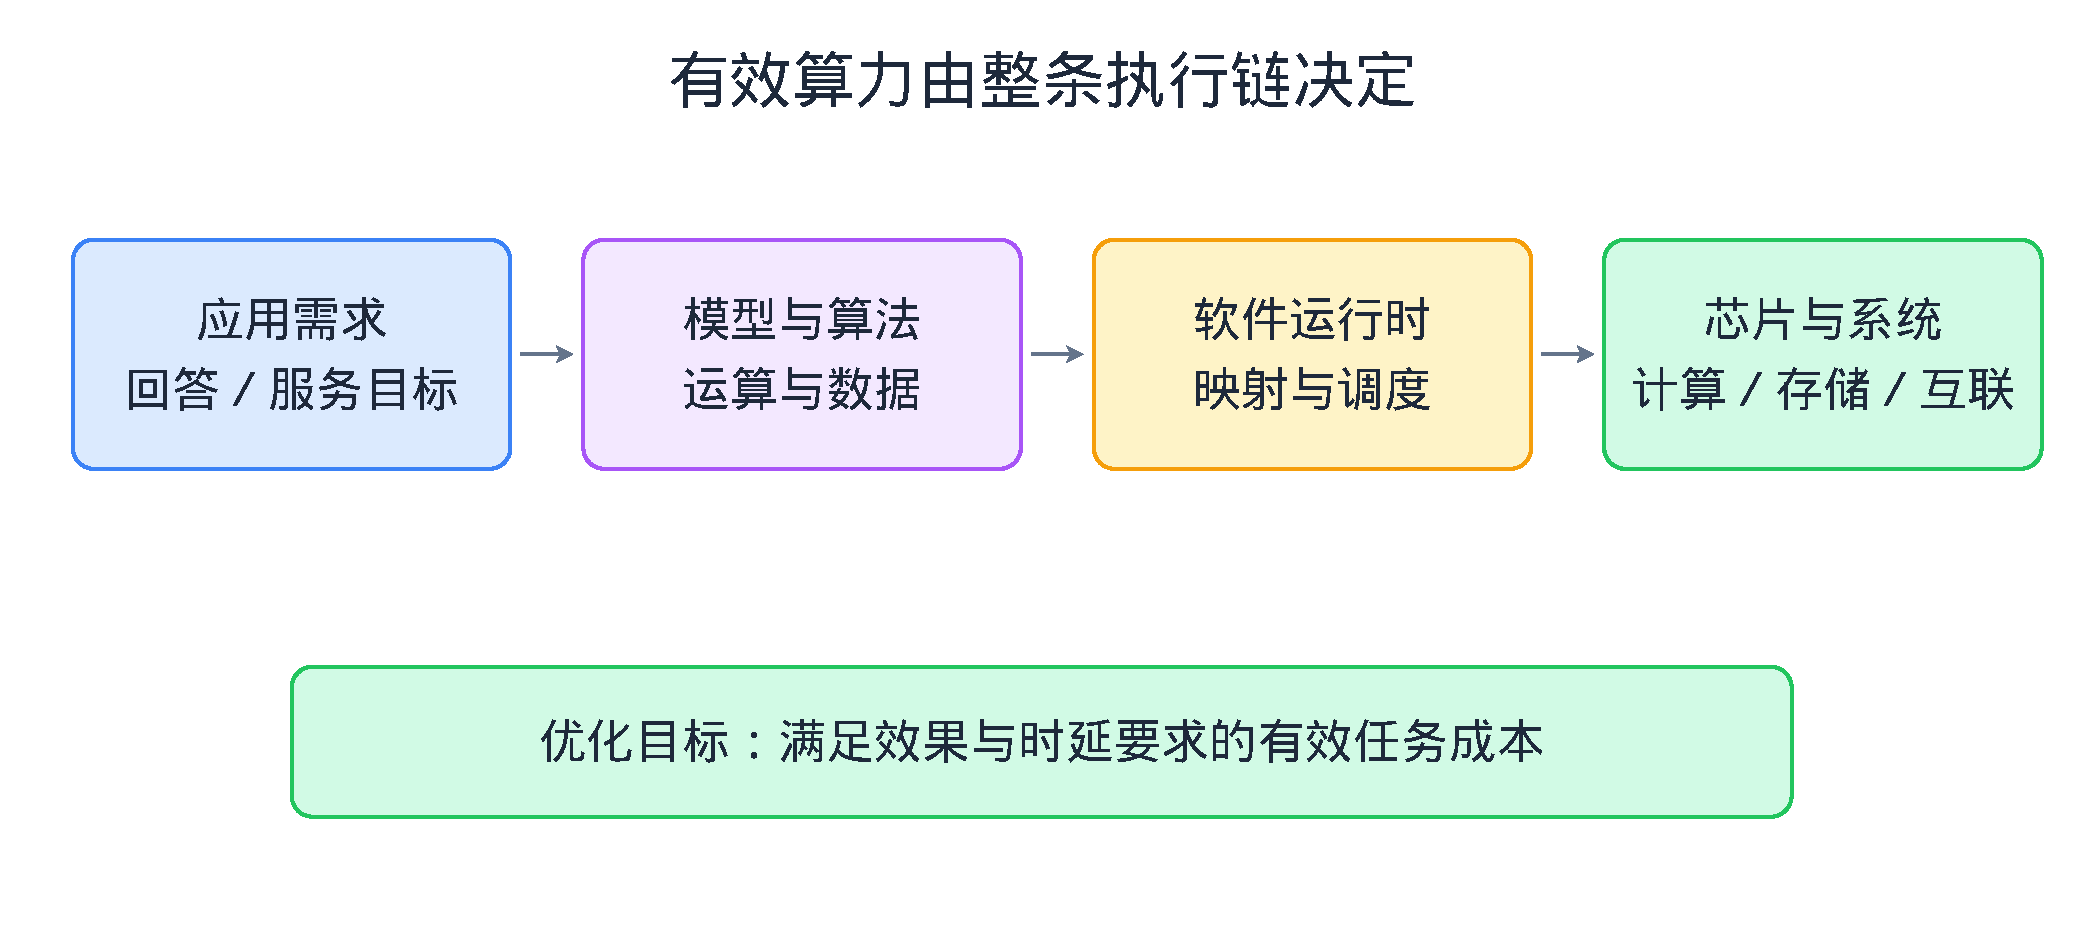
\includegraphics[width=\linewidth,height=.68\textheight,keepaspectratio]{assets/figure-01.pdf}
\caption{有效算力由整条执行链决定，依据节目口述整理（00:01:10–00:13:10）}
\end{figure}
\begin{knowledgebox}{读图：从造芯片到优化系统：算力问题的边界}
图 1 上方由左向右排列四个模块，并以单向箭头依次连接：最左侧为“应用需求（回答／服务目标）”，向右指向“模型与算法（运算与数据）”，再指向“软件运行时（映射与调度）”，最终落到最右侧的“芯片与系统（计算／存储／互联）”。在这条四级链路下方，横跨设置了一个总结框，标明“优化目标：满足效果与时延要求的有效任务成本”，说明上层任务需经模型与运行时转换后才能成为芯片上的实际动作。
\end{knowledgebox}
这印证了本章的核心论点：讨论造芯还是做软件优化，都必须回到整条执行链条上，以实际任务的交付效果、时延与综合成本作为衡量标准。
\needspace{6\baselineskip}\subsection{本章小结}
本章顺着肖志斌从浙大、UC Davis 到 Oracle、阿里再到创立 ZFlow.AI 的二十余年经历，展示了计算架构如何随时代负载而演进。无论是早期的众核片上数据流，还是将数据库算子硬化进 SPARC 处理器以用满内存带宽，核心都是通过软硬件协同消除系统瓶颈。当单芯片工艺红利放缓、大模型集群高昂的硬件成本阻碍试错时，算力优化的重点转向系统级仿真、编译与运行时调度；而唯有当特定应用与模型架构趋于稳定时，通过金属层修正或专用算子硬化去定制芯片才具备经济合理性。
\needspace{8\baselineskip}\section{一颗芯片如何走向量产}
上一章我们看到，当通用算力逼近工艺红利边界、模型架构与特定场景逐渐稳定时，定制专用芯片在经济学上才真正成立。然而从“决定造一颗芯片”到“服务器真正上线运行”，中间横亘着一条漫长且容错率很低的工程链条。本章顺着肖志斌在芯片研发一线的实践经验（00:13:10），拆解一颗芯片如何从最初的市场需求定义，历经架构权衡、逻辑实现、验证仿真与晶圆制造，一步步走向量产，并探讨 AI 工具与现场可编程门阵列（FPGA）在其中扮演的角色。
\needspace{6\baselineskip}\subsection{需求、架构与逻辑设计}
任何芯片工程的起点都不是直接画电路，而是像建房子一样先明确需求：究竟是做音视频编解码芯片、特定标准的 Wi-Fi 通信芯片，还是做 CPU、GPU 这类相对通用的计算芯片。肖志斌指出，这一步由市场或特定应用场景驱动。例如超大规模云服务商（hyperscaler）或大型视频流平台，每天要面对手机上传的各种视频格式，必须先通过转码（transcoding）存成服务器上的统一格式，分发时再根据不同终端的解码能力与分辨率转成不同格式。许多通用 CPU 并不具备高效的专用编解码硬件，如果纯粹靠堆叠 CPU 服务器来承担转码，总拥有成本（TCO，Total Cost of Ownership）会很高，这就催生了定制视频转码芯片的需求。

在研发周期上，过去做一颗传统 CPU 芯片，仅设计周期就要两年，加上流片、系统集成与软件适配，最终上线往往耗时三到五年。近年来英伟达将行业发布节奏带快，看起来每年都在发布新芯片，甚至一年推出数款，但这并不意味着单颗芯片的完整研发周期缩短到了一年。实际上，英伟达内部采用了多代团队交错重叠（overlap）的并行开发模式：单颗芯片从设计到开发依然需要两年左右，今天看到的 B300、GB300 等产品，其立项与设计工作早在两三年前就已经启动。正因为芯片从立项到面市存在两三年的时间差，且市场竞争激烈——第一名占据大部分市场，第二名占小部分，第三、第四名往往难以分到份额——芯片定义阶段必须包含深入的市场与竞品调研，确保产品在两三年后依然具备竞争力。

当业务需求与商业账算清楚后，架构师正式入场（00:14:34）。架构师的核心任务是在\textbf{功耗、性能、面积（PPA，Power, Performance, Area）以及成本（cost）}之间做权衡（trade-off），确定芯片尺寸与功能边界，最终输出芯片的顶层规格说明（spec，包含指令集或高层级模块结构定义）。随后，微架构师接手，在架构师给定的约束条件（constraint）下，将抽象规格转化为可实现的硬件微架构。以编解码中的快速傅里叶变换（FFT）为例，同一个数学功能有多种硬件实现方式，每种方式的 PPA 权衡各不相同；微架构师选定具体实现方案后，自己或配合前端设计工程师，使用硬件描述语言（如 Verilog 或 SystemVerilog，节目口述中通俗地称作“硬件编程语言”）编写寄存器传输级（RTL，Register Transfer Level）的设计描述。

\needspace{6\baselineskip}\subsection{验证、物理设计、流片和测试}
RTL 设计描述完成后，研发便进入验证与后端实现阶段。从工程链路来看，一颗芯片从逻辑描述走向量产需要跨越六个相互衔接的步骤：
\begin{enumerate}
\item 多维验证与硬件仿真（emulation）；
\item 逻辑综合与物理设计（布局布线、时钟与供电协同）；
\item 送交晶圆代工厂制作掩膜并完成晶圆流片；
\item 晶圆级缺陷测试与裸片（die）切割；
\item 芯片封装与印制电路板（PCB）系统级测试；
\item 客户送样与规模化量产。
\end{enumerate}

在这条链路中，验证（verification）往往消耗庞大的人力与算力成本（00:16:39）。肖志斌提到，在没有引入 AI 辅助之前，一家芯片设计公司里设计工程师与验证工程师的人数配比通常达到 1:2 甚至 1:3。芯片验证绝不仅是编写简单的测试平台（testbench），验证团队需要完成功能验证、形式验证、时序验证与物理验证；在芯片尚未流片制造出来之前，还必须利用现场可编程门阵列（FPGA，Field-Programmable Gate Array）或购买楷登电子（Cadence）的 Palladium 等大型专用硬件仿真平台进行系统级仿真。嘉宾指出，如果芯片流片失败，不仅意味着数亿美元的资金投入可能损失，还会导致一两年的研发时间窗口丧失。

为了说明验证工具对芯片公司的生死意义，肖志斌分享了英伟达早期的一个行业故事：当年黄仁勋在研发早期 GPU 时，公司资金几乎见底，但他依然拿出最后那笔钱购买了一台昂贵的硬件仿真器专门用于芯片验证。在验证工具匮乏的年代，芯片往往要反复流片好几次才能成功；正是依靠这台仿真器在流片前扫清逻辑缺陷，英伟达才得以实现关键产品的一次性流片成功。直到今天，成熟的验证与仿真手段依然是行业生命线，完善的验证与仿真能降低流片失败的风险；部分设计问题可以通过局部金属层修正（metal fix）处理，是否需要重新流片取决于具体缺陷。

当 RTL 通过验证并经逻辑综合转化为门级网表后，后端团队会完成布局布线（place and route）、时钟（clocking）与供电（power）设计，并与系统厂商就供电导入和封装（package）方案开展协同设计（co-design）。版图交付给台积电或中芯国际等晶圆代工厂（foundry）后，便进入约 3 到 4 个月的制造期：代工厂根据版图制作掩膜（mask），像印刷一样在硅晶圆上一层层曝光加工，现代复杂芯片的掩膜层数往往达到几十层甚至接近上百层。三四个月后晶圆（wafer）出厂，先通过晶圆测试筛查电性与功能等缺陷（defect），再切割成单颗裸片（die），并根据测试结果筛选合格裸片；合格的裸片送交封装厂完成封装，随后贴装到系统厂商的 PCB 板卡上，完成实验室环境下的功能与系统软硬件联调测试，最终向客户送样并导入量产。

\needspace{6\baselineskip}\subsection{AI 能帮设计者完成哪些工作}
面对这条长周期、低容错的研发链路，硅谷已有不少创业公司与大厂开始尝试引入智能体（agent）来协助芯片设计与验证工作（00:21:20）。肖志斌观察到，目前 AI 在芯片研发中应用较多的环节主要有两块：第一块是芯片验证，因为验证工作具有明确的输入与输出，且背后有仿真工具可以检验结果是否出错，其模式接近编程智能体（coding agent），因此用 AI 辅助验证的项目很多，但 AI 参与验证只是提升效率的手段，并不等于芯片可以省去工程验证；第二块是后端物理设计，诸如芯片布局规划（floorplan）与布局布线，新思科技（Synopsys）、楷登电子（Cadence）等电子设计自动化（EDA，Electronic Design Automation）厂商已经在工具链中大量使用了 AI 算法。

相比之下，用 AI 直接做从 0 到 1 的正向设计目前还相对较少，而在更上游的架构定义阶段——即决定做什么芯片、如何定义顶层规格与权衡 PPA——现成的自动化工具依然匮乏，仍依赖人类架构师的经验与判断。此外，肖志斌指出当前传统芯片公司引入 AI 面临一层组织阻力：成熟芯片企业都有一套既有的研发流程，许多工程师不愿用 AI 取代自己现有的工作环节，导致 AI 在大多数传统芯片公司里仅扮演辅助角色。

基于这一观察，嘉宾提出了一个个人判断：下一代最优秀的芯片公司，很可能是一家原生围绕人工智能构建（AI-native）的芯片设计公司。在他看来，要把 AI 的价值充分发挥出来，不能只在旧流程上做局部修补，而需要从架构探索、逻辑设计、验证仿真到物理实现的全流程，都用 AI 原生的方式去组织研发；没有历史流程包袱的新兴团队，更容易推动这种全流程变革。

在本节末尾，节目还讨论了工程界对 FPGA 芯片的常见疑问：为什么近两年在主流 AI 数据中心推理中较少听到 FPGA（00:24:55）？肖志斌解释说，当主流大模型的计算负载（workload）固定下来后，FPGA 并不是数据中心推理最高效的实现方式；但在那些对现场可编程性要求高、通信协议随时变化或场景碎片化的领域，FPGA 依然被大量使用——从流片前的硬件仿真（emulation），到芯片间协议未定型时的互联适配，FPGA 仍在承担重要的工程支撑角色。

\begin{importantbox}{芯片研发中的 PPA 权衡与前端验证配比}
\begin{enumerate}
\item PPA（Power, Performance, Area）与 Cost：架构师定义芯片规格的核心标尺，分别对应功耗、性能、芯片面积与成本，任何架构方案都是在四者之间寻找贴合目标场景的工程折中。
\item 设计与验证配比（1:2 至 1:3）：在传统芯片研发团队中，每配置 1 名完成 RTL 设计的前端工程师，通常需要配套 2 到 3 名验证工程师，开展功能、形式、时序与物理验证，并结合 FPGA 与 Palladium 等硬件仿真器排查缺陷，以降低流片失败风险。
\end{enumerate}
\end{importantbox}
\begin{knowledgebox}{为什么英伟达能做到“每年出新芯片”？}
一颗现代复杂芯片从架构定义、设计验证到流片量产，单代完整研发周期通常需要 2 年左右（传统 CPU 甚至长达 3 到 5 年）。英伟达之所以能呈现出“一年一代甚至一年多款”的极速迭代节奏，核心在于其内部采用了多代研发团队交错重叠（overlap）的并行开发模式：当一代芯片进入后端流片与系统点亮时，下一代甚至下下一代芯片的架构与微架构设计早已在两三年前提前启动。
\end{knowledgebox}
\begin{table}[H]\centering\small
\caption{芯片从立项到量产的关键工程阶段与核心任务}
\begin{tabular}{>{\raggedright\arraybackslash}p{\dimexpr(\linewidth-6\tabcolsep)/3\relax}>{\raggedright\arraybackslash}p{\dimexpr(\linewidth-6\tabcolsep)/3\relax}>{\raggedright\arraybackslash}p{\dimexpr(\linewidth-6\tabcolsep)/3\relax}}
\toprule
研发阶段 & 核心参与角色 & 解决的核心问题与关键动作\\\midrule
需求与架构定义 & 产品团队、系统架构师 & 瞄准高 TCO 痛点（如云端视频转码），完成竞品调研、PPA 与成本权衡，输出芯片顶层规格（Spec）。\\[4pt]
微架构与逻辑设计 & 微架构师、前端设计工程师 & 在架构约束下选定具体算法硬件实现路径（如 FFT 结构），使用硬件描述语言完成寄存器传输级（RTL）设计。\\[4pt]
多维验证与仿真 & 验证工程师（配比约占 2/3） & 执行功能、形式、时序与物理验证，利用 FPGA 或 Palladium 硬件仿真平台扫清逻辑缺陷，确保一次流片成功。\\[4pt]
物理设计与晶圆制造 & 后端工程师、晶圆代工厂 & 完成逻辑综合、布局布线、时钟与供电协同设计；交付版图至代工厂历经近百层掩膜曝光，耗时 3–4 个月产出晶圆。\\[4pt]
封装测试与系统量产 & 测试厂、封装厂、系统工程师 & 筛查晶圆缺陷并切割裸片（Die），完成芯片封装与 PCB 系统板级联调测试，向客户送样并导入大规模量产。\\[4pt]
\bottomrule\end{tabular}\end{table}
在理解了为何芯片研发周期动辄耗时两三年、且流片前必须投入大量人力做验证与仿真之后，我们可以通过图 2 将前端设计、后端实现与制造测试的工程步骤串联起来。
\begin{figure}[H]\centering
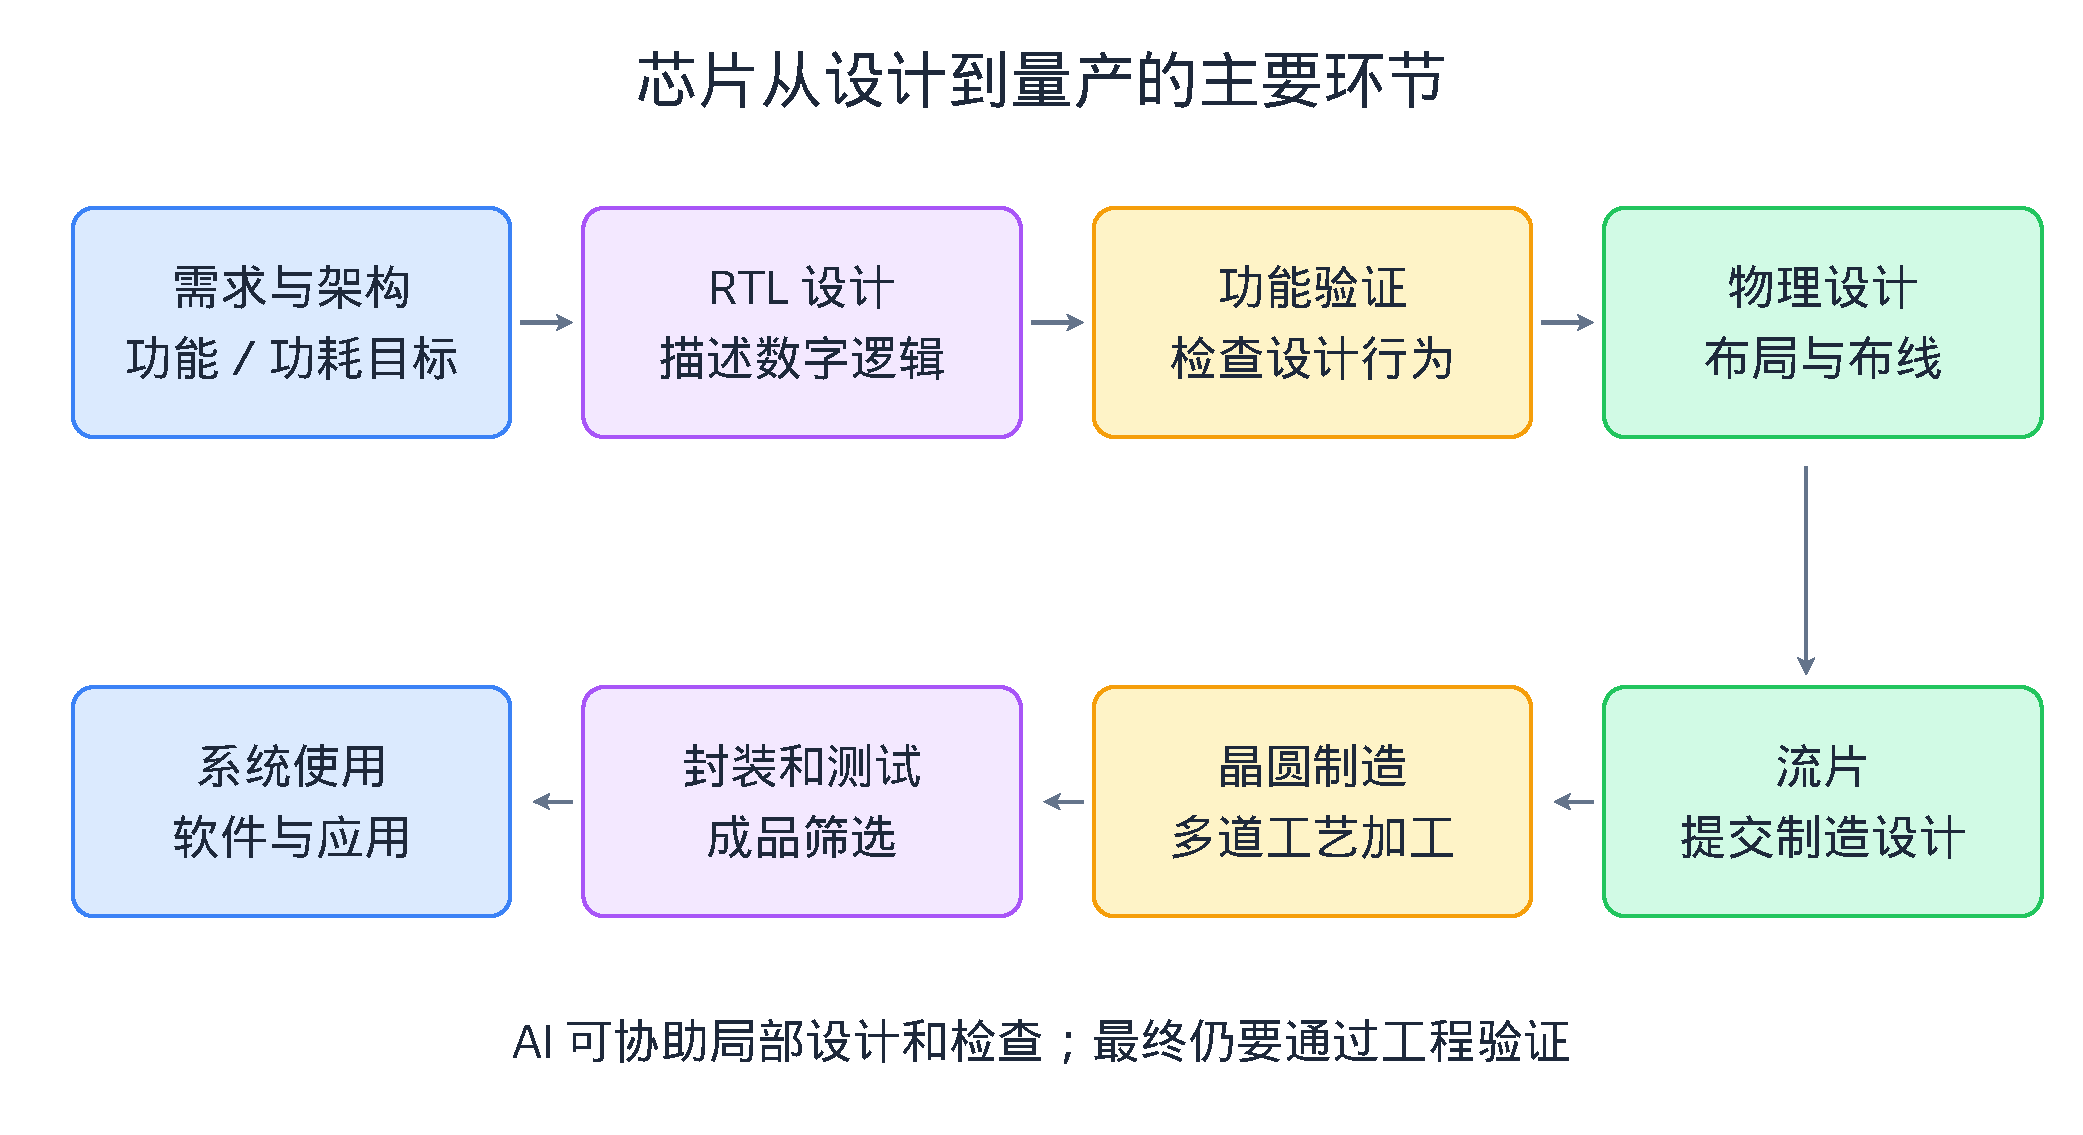
\includegraphics[width=\linewidth,height=.68\textheight,keepaspectratio]{assets/figure-02.pdf}
\caption{芯片从设计到量产的主要环节，依据节目口述整理（00:13:10–00:25:50）}
\end{figure}
\begin{knowledgebox}{读图：一颗芯片如何走向量产}
图 2 分为上下两行共八个环节。上行从左至右依次为“需求与架构（功能／功耗目标）”\ensuremath{\rightarrow}“RTL 设计（描述数字逻辑）”\ensuremath{\rightarrow}“功能验证（检查设计行为）”\ensuremath{\rightarrow}“物理设计（布局与布线）”。随后箭头从上行最右侧的“物理设计”向下指向下行最右侧的“流片（提交制造设计）”，再自右向左依次经过“晶圆制造（多道工艺加工）”\ensuremath{\rightarrow}“封装和测试（成品筛选）”\ensuremath{\rightarrow}“系统使用（软件与应用）”。图底部文字指出：“AI 可协助局部设计和检查；最终仍要通过工程验证”。
\end{knowledgebox}
从图 2 的双向折返链路可以看出，芯片研发环环相扣，AI 工具虽能加速局部设计与检查，但仍需依靠完整的工程验证来规避流片与系统集成风险。
\needspace{6\baselineskip}\subsection{本章小结}
本章呈现了一颗芯片从市场需求走向规模量产的工程全貌：研发始于对高 TCO 场景（如大规模视频流转码）的需求分析，经架构师完成 PPA 权衡与微架构师完成 RTL 设计后，需投入两三倍于设计人力规模的验证团队，借助多维验证、FPGA 与硬件仿真器保障一次流片成功；随后历经综合、布局布线、代工厂三四个月的几十至近百层掩膜制造、切割封装与板级测试，单代研发通常耗时两年以上。AI 工具已在验证与物理设计环节落地，而嘉宾认为全流程采用 AI 原生方式的组织有望在未来脱颖而出。
\needspace{8\baselineskip}\section{全球供应链、指令集与纳米制程}
上一章我们拆解了一颗芯片从场景需求定义、微架构设计、大规模验证到流片封装的完整研发流程。然而，任何一家芯片公司都无法在真空中独自跑完这条耗时两三年的长链路。本章我们将视野从单颗芯片的工程内部扩展到支撑它的全球半导体生态：剖析设计、制造、设备与 EDA（电子设计自动化）工具的跨国分工，探讨开放指令集 RISC-V 的真实边界，并揭开“七纳米到二纳米”制程演进背后的物理本质——功耗、密度与片上存储器的缩放瓶颈。
\needspace{6\baselineskip}\subsection{设计、制造、设备与封装的分工}
从单颗芯片的验证工具延伸到全球半导体产业格局，主持人提问：“美国擅长芯片设计、台积电擅长芯片制造”这一常见说法是否准确（00:25:51）？肖志斌给出了肯定的判断，并进一步将美国在上游的优势拆解为两块：第一是芯片设计知识产权（IP）与 EDA 工具，第二是架构与芯片设计。

EDA 即电子设计自动化，是贯穿芯片研发各环节的专用工业软件体系。在 Synopsys（新思科技）、Cadence（楷登电子）和 Mentor Graphics（明导国际，现属 Siemens EDA）三大厂商构建的工具链下，芯片研发的每个工种都配有专门的软件支撑（00:27:00）：
\begin{enumerate}
\item 架构设计：工具相对较少，代表有 Synopsys 的系统架构仿真工具 Platform Architect Ultra（PAU）；
\item 逻辑综合与仿真：将 RTL 设计转化为门级网表的逻辑综合（synthesis）工具，以及做 RTL 验证的逻辑仿真（simulation）工具（如 VCS）；
\item 物理与后端验证：负责布局布线（place and route）的物理设计工具、时序（timing）验证工具、形式验证工具以及封装设计（package design）工具。
\end{enumerate}

为什么这些昂贵的 EDA 工具高度集中在这三家公司手中，其他企业难以轻易替代？嘉宾指出了背后的两个原因。其一是历史上的大规模兼并收购（merger and acquisition），三大厂商在数十年间并购整合了许多拥有细分算法的小型创业公司，沉淀了大量知识产权；其二是与晶圆代工厂（foundry）的协同设计（co-design）。后端物理设计工具并非脱离制造工艺独立编写的代码，而是与台积电等晶圆代工厂的工艺节点同步共同开发出来的，凝聚了制造端的合作经验。

放眼全球，半导体供应链（supply chain）是一条漫长且高度专业化分工的网络（00:29:06）。肖志斌解释，晶圆代工厂（foundry）主要指台积电、中芯国际（SMIC）这类代工制造硅芯片的企业；而在整个制造端，除了逻辑芯片代工厂外，还有生产存储器的晶圆厂——例如中国大陆有长鑫、长存等布局动态随机存取存储器（DRAM）与非易失性闪存（NAND）的存储制造企业，同时也有本土的 EDA 与 FPGA 公司。总体来看，中美两国的半导体产业链门类最为齐全；与此同时，其他国家和地区也掌握着关键环节：英国拥有移动端广泛采用的 Arm 指令集 IP；荷兰 ASML（阿斯麦）制造高端光刻机；日本拥有东京电子等半导体设备商及核心材料供应商；韩国则在存储器制造与代工领域占据重要地位。

\needspace{6\baselineskip}\subsection{开源指令集为什么不等于现成芯片}
在全球供应链的讨论中，主持人提到了加州大学伯克利分校的开源传统：伯克利不仅在软件层开源了 vLLM、SGLang 等大模型推理服务框架，在硬件层还推出了开放指令集架构 RISC-V，这背后的初衷是什么（00:30:30）？肖志斌回忆了与 RISC-V 创始团队成员的交流：早年学者们在做计算机体系结构研究与开发时，若想使用主流的 Arm 架构，不仅涉及商业授权许可（license）模式与相关费用，而且 Arm 当时主要面向移动端（mobile）应用，对学术研究而言自由度不够高。因此，伯克利团队决定从头设计一套开放、可扩展性好且没有历史遗留（legacy）兼容包袱的新指令集，以面向新的工作负载。

如今，RISC-V 已经在工业界得到了广泛采用。肖志斌提到一个许多软件开发者不常注意的事实：在英伟达（NVIDIA）自家的 GPU 芯片内部，许多控制器和辅助处理器其实都采用了 RISC-V 架构。围绕这一生态，全球形成了 RISC-V 峰会（Summit）与产业联盟：美国有以 SiFive 为代表的企业，中国台湾有专注于 RISC-V IP 的晶心科技（Andes），中国大陆也有许多包括阿里系校友在内的创业团队投入其中。嘉宾谈到，即便在地缘政治紧张的背景下，全球芯片同行在开源生态上的配合与合作依然很多。

不过，从工程实现的角度需要明确区分三个不同层次：\textbf{开放指令集架构（ISA）、开源具体硬件实现与芯片物理制造}。RISC-V 开放的是软件与硬件之间的指令集规范，免除了指令集架构层的授权限制与历史兼容包袱；但要把纸面上的规范变成数据中心可用的实体芯片，企业依然需要编写或采购微架构 RTL 实现，购买高速接口如串行器/解串器（SerDes）等商业闭源 IP，支付 EDA 软件许可费，并在晶圆代工厂投入资金完成流片与封装测试。因此，开放指令集并不等于零成本的现成开源芯片。

\needspace{6\baselineskip}\subsection{从七纳米到二纳米：能效、密度与成本}
理清了产业链与指令集后，访谈进入了大众常听闻却容易误解的概念——“7 纳米、5 纳米、3 纳米、2 纳米”制程工艺（00:33:04）。肖志斌指出，在大约 65 纳米节点以前，“几纳米”确实对应着晶体管（transistor，包含源极 source、漏极 drain 和栅极 gate）的一个物理尺寸，即栅长（gate length）。但在 65 纳米之后，节点数字更多演变成了一个代表“整代工艺技术”的商业与营销命名，不再直接对应某一个单一的物理长度。而且，不同厂商（如台积电、三星、英特尔）各自命名的“7 纳米”之间也没有直接的尺寸可比性，业界横向比较看的仍是特定设计下的 PPA（功耗、性能、面积）表现。在实际工程中，代表一代工艺技术的常见参数包括：
\begin{enumerate}
\item 晶体管结构形态：例如在先进工艺中演进出的三维立体鳍式场效应晶体管（FinFET，不同代际会采用新型晶体管结构，不能将 FinFET 简单泛化等同于所有 2 纳米工艺）；
\item M0 pitch（最底层金属间距）：硅片上方最底层金属互连线相邻重复结构的间距（pitch 指中心间距，不等于单根线宽，尽管口述中有时简称为宽度）；
\item Standard cell（标准单元）尺寸：构成与门、或门等基本逻辑门电路的标准单元面积与 PPA；
\item SRAM（片上静态随机存取存储器）密度：单位面积内能集成的片上存储容量与单元尺寸。
\end{enumerate}

那么，工艺制程从 7 纳米演进到 5 纳米、3 纳米乃至 2 纳米，主要解决了什么问题？肖志斌强调了一个容易被外界忽视的结论：\textbf{制程演进的重点不在于单纯让芯片运行速度（频率）变快，而在于降低功耗}（00:35:59）。在工程比较中通常有两种口径：一是在同等性能水平下对比功耗能降低多少，二是在同等功耗预算下对比性能可提升多少。嘉宾指出，每一代制程演进在降低同等性能下的功耗方面带来的收益，明显大于单纯提升运行频率的幅度。

从电路物理机制来看，芯片的总功耗由动态功耗和静态功耗两部分构成：
\[
P_{\text{total}} = P_{\text{dynamic}} + P_{\text{static}}
\]

其中，\(P_{\text{total}}\) 表示芯片总功耗，\(P_{\text{dynamic}}\) 表示逻辑门在开与关状态切换（充放电）过程中产生的动态功耗，\(P_{\text{static}}\) 表示晶体管处于稳定开关状态下因漏电流产生的静态功耗。早年遵循登纳德缩放（Dennard scaling），供电电压（supply voltage）能随着晶体管尺寸缩小而同步降低；但随着工艺继续微缩，晶体管受限于开启所需的基准电压，供电电压无法无限下降，漏电流效应逐渐凸显，静态功耗占比随之上升。即便如此，先进制程带来的整体功耗下降依然具有重要的系统价值：单颗芯片功耗降低意味着发热量减少，数据中心在供电与散热受限的单个机架（rack）内就能部署更多算力，从而提升单机柜的计算密度，并减少跨机柜的数据搬运。

与此同时，肖志斌指出了先进制程演进中另一个影响 AI 芯片架构的现象：逻辑电路与片上存储器的缩放比例并不同步（00:39:19）。在许多 AI 芯片中，逻辑计算单元与片上静态随机存取存储器（SRAM）各占相当一部分芯片面积（嘉宾在口述中以“一半是逻辑、一半是 SRAM”作为典型举例，实际不同架构芯片的面积配比各有不同）。但在从 5 纳米向 3 纳米及更先进节点演进的过程中，逻辑部分仍能继续微缩，而片上 SRAM 单元尺寸（cell size）的缩放收益已明显趋缓、基本停下。这对于大模型推理服务（serving）意味着什么？在推理过程中，预填充（prefill）阶段偏重并行计算，仍能直接受益于逻辑电路的微缩；而逐词元解码（decode）阶段在许多场景下受制于内存访问（memory-bound）。对于像 Groq、Cerebras 这类高度依赖大容量片上 SRAM 的芯片架构而言，当 SRAM 难以继续随工艺按原比例缩小时，其芯片设计哲学、逻辑与存储的面积配比就需要调整，或者转向 3D 堆叠等其他技术路径。

\begin{warningbox}{常见误区：制程节点数字与片上 SRAM 的缩放边界}
65 纳米之后的“7nm/5nm/3nm/2nm”不再直接等于晶体管的实际栅长，而是综合了晶体管结构、最底层金属间距（M0 pitch）、标准单元面积与 SRAM 密度的工艺代际名称。制程升级的核心收益在于同等性能下降低功耗（或同等功耗下提升性能），借此降低散热压力、提升数据中心单机架（rack）的计算密度。同时需要注意，逻辑电路与片上存储并非按同一比例缩小：在 5nm 向 3nm 演进时，片上 SRAM 的尺寸缩放已明显放缓。对于依赖大容量片上 SRAM 应对内存访问瓶颈的 AI 芯片而言，这意味着单纯等待制程升级无法自动换来同比例的片上容量增长，必须结合架构配比调整或 3D 堆叠等方案。
\end{warningbox}
\begin{knowledgebox}{工程背景：为什么开源 RISC-V 与买齐 EDA 仍造不出低成本芯片}
许多软件背景的读者容易将硬件领域的 RISC-V 类比为 Linux 或 vLLM 等可直接部署的开源软件。实际上，RISC-V 开放的是“指令集架构（ISA）”这一软硬件接口规范，免除了类似 Arm 的架构授权限制与历史兼容包袱。要将其变为实体芯片，研发团队仍需完成微架构设计、采购商业外围 IP（如高速通信接口 SerDes），并依赖 Synopsys、Cadence、Mentor Graphics（现属 Siemens EDA）三大厂商的 EDA 工业软件完成综合与布局布线，最后交由晶圆代工厂流片。EDA 工具之所以壁垒深厚，既源于数十年的并购积累，也因为其后端物理设计工具是与代工厂的制造工艺协同开发（co-design）出来的。
\end{knowledgebox}
\begin{table}[H]\centering\small
\caption{全球半导体生态核心环节与工程壁垒对比}
\begin{tabular}{>{\raggedright\arraybackslash}p{\dimexpr(\linewidth-6\tabcolsep)/3\relax}>{\raggedright\arraybackslash}p{\dimexpr(\linewidth-6\tabcolsep)/3\relax}>{\raggedright\arraybackslash}p{\dimexpr(\linewidth-6\tabcolsep)/3\relax}}
\toprule
核心环节与概念 & 解决的工程问题 & 核心机制与现实制约\\\midrule
EDA（电子设计自动化） & 支撑从架构仿真、逻辑综合、验证到物理布局布线的全流程研发 & 由 Synopsys、Cadence、Mentor Graphics（现属 Siemens EDA）主导；通过历史并购积累知识产权，且后端工具需与代工厂工艺协同设计（co-design）\\[4pt]
晶圆制造、存储与设备材料 & 将芯片物理版图通过近百层掩膜与光刻制造为实体硅晶圆 & 晶圆代工（如台积电、中芯国际）、存储器制造、设备与材料全球分工（如 ASML 光刻机、日本设备与材料）；受扩产周期与设备交付量限制\\[4pt]
RISC-V（开放指令集架构） & 摆脱闭源指令集的高昂授权费与历史包袱，支持灵活自定义扩展 & 源自伯克利；已广泛用于控制器及 GPU 内部辅助核，但仅开源指令规范，微架构实现、商业 IP 与流片仍需高昂成本\\[4pt]
先进制程节点（7nm 至 2nm） & 在同等性能下大幅降低芯片功耗，从而提升机架级计算密度 & 数字已非实际栅长；虽能继续微缩逻辑电路并改善能效，但在先进节点上面临片上 SRAM 缩放趋缓的物理制约\\[4pt]
\bottomrule\end{tabular}\end{table}
针对工程讨论中常把“开源指令集”等同于“免费现成芯片”、或把“纳米节点名称”直接当作单一物理尺寸的误解，图 3 按自上而下的技术层次划分了从软件接口到物理制造的边界。
\begin{figure}[H]\centering
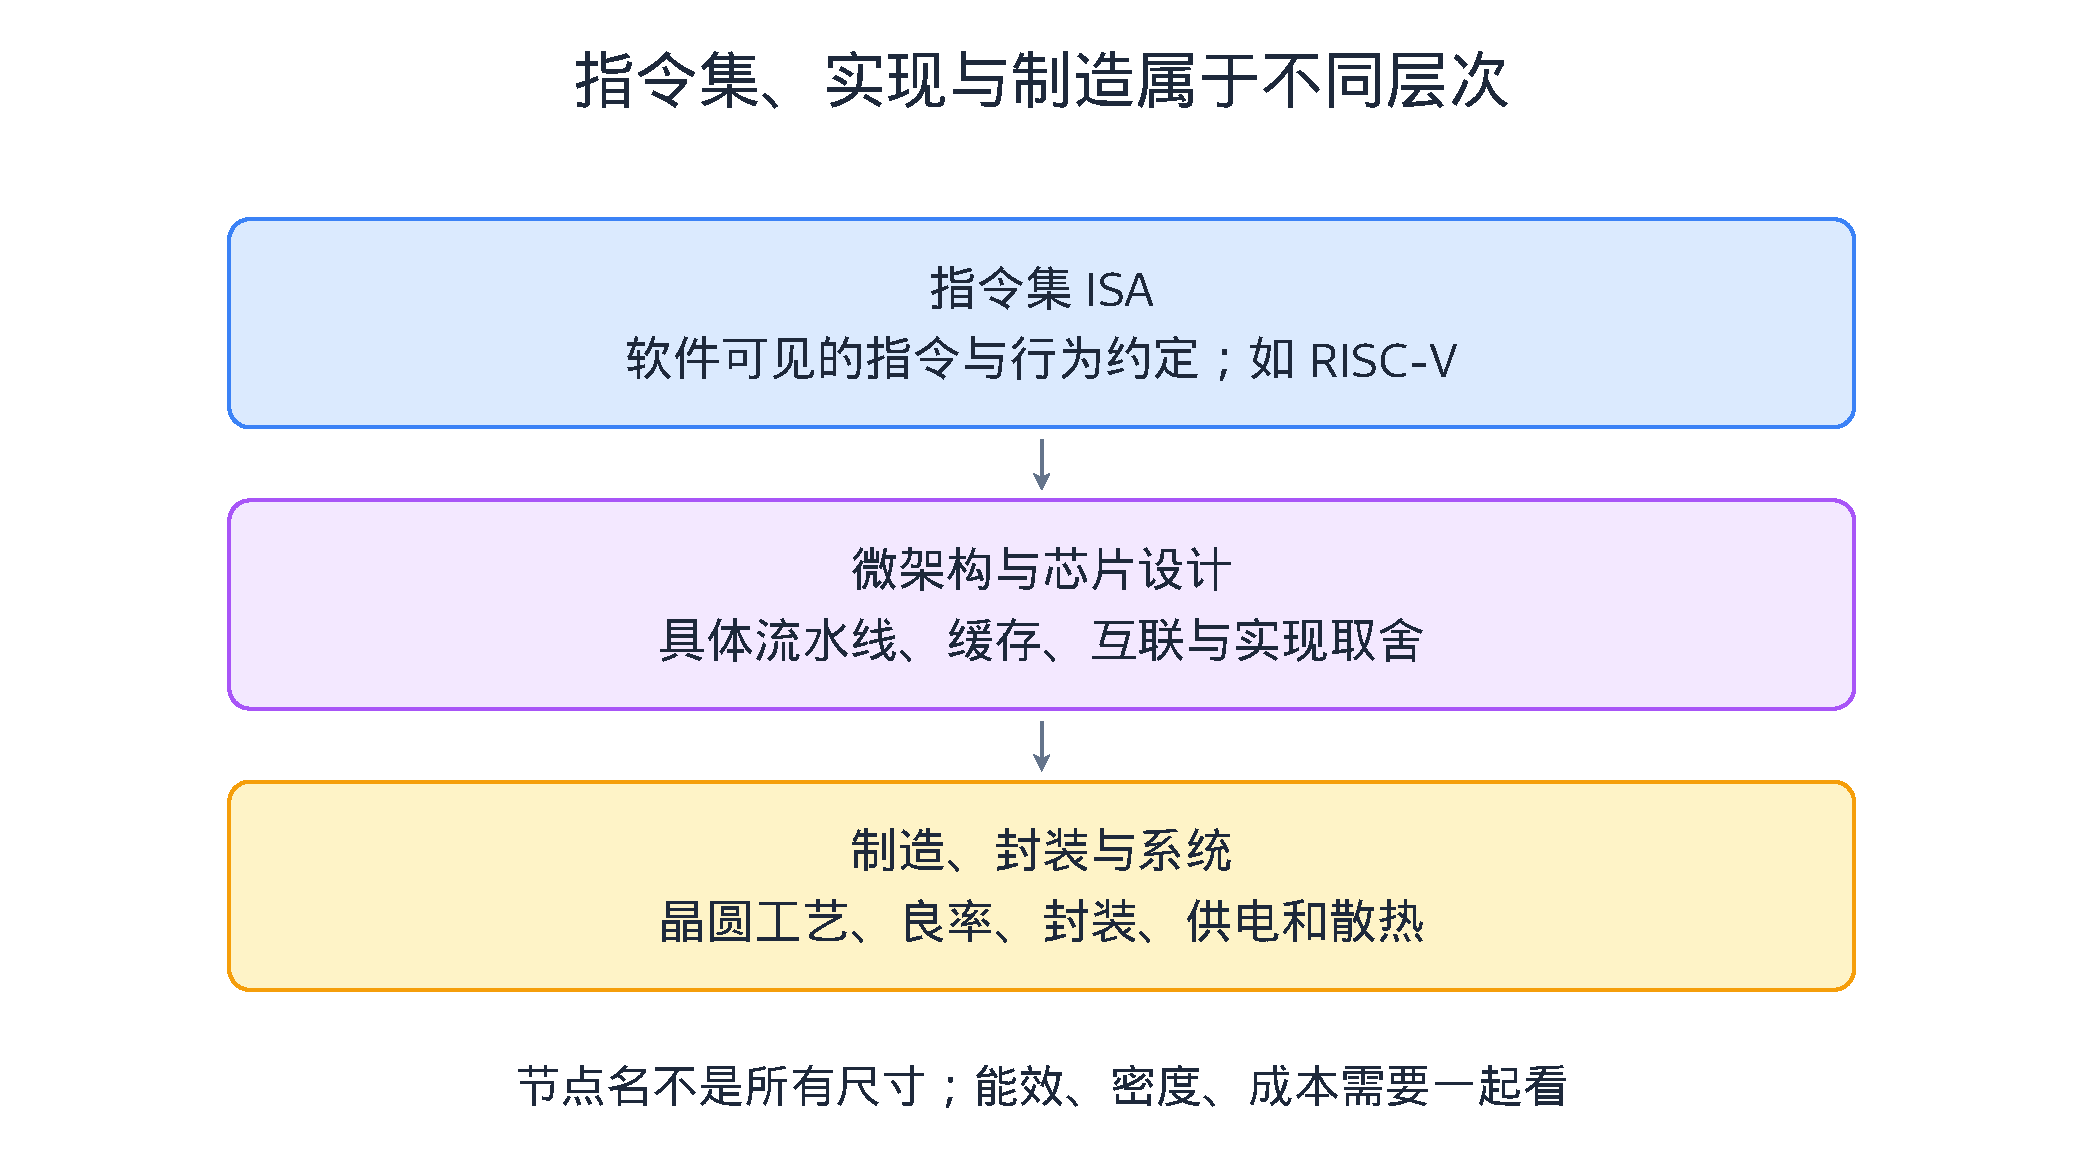
\includegraphics[width=\linewidth,height=.68\textheight,keepaspectratio]{assets/figure-03.pdf}
\caption{指令集、实现与制造属于不同层次，依据节目口述整理（00:25:50–00:40:55）}
\end{figure}
\begin{knowledgebox}{读图：全球供应链、指令集与纳米制程}
图 3 主体为自上而下垂直排列并通过箭头顺次连接的三个宽框：顶层是“指令集 ISA（软件可见的指令与行为约定；如 RISC-V）”；中间层是“微架构与芯片设计（具体流水线、缓存、互联与实现取舍）”；底层是“制造、封装与系统（晶圆工艺、良率、封装、供电和散热）”。最下方一行文字总结道：“节点名不是所有尺寸；能效、密度、成本需要一起看”。
\end{knowledgebox}
图 3 清晰表明，RISC-V 仅开放了顶层的软件接口约定，企业仍需承担中间层的微架构实现与底层的制造封装成本；同样，评判工艺节点也必须综合考察能效、密度与系统成本。
\needspace{6\baselineskip}\subsection{本章小结}
本章将芯片研发置于全球半导体工业体系中进行审视：一颗芯片的诞生依赖跨国供应链的分工配合——美国在架构、IP 与三大 EDA 厂商工具链上占据优势，中国大陆、中国台湾与韩国等地布局逻辑代工与存储器制造，荷兰与日本则在光刻机、设备与材料上握有关键环节。伯克利发起的 RISC-V 开放指令集虽减少了指令集层的授权束缚并已用于 GPU 内部控制器，但并未省去微架构实现、商业 IP、EDA 协同与晶圆制造的工程成本。而在制造端，从 7 纳米向 2 纳米演进的核心价值在于降低同等性能下的功耗，以提升数据中心单机柜的计算密度；同时，先进节点上片上 SRAM 与逻辑电路无法按同一比例微缩，也给依赖片上存储的 AI 芯片架构带来了新的设计约束。
\needspace{8\baselineskip}\section{大模型推理在忙什么：计算、搬运与等待}
上一章我们看到，从 7 纳米向 2 纳米演进的核心收益在于降低功耗、提升单机柜计算密度，而先进节点上片上静态随机存取存储器（SRAM）缩放趋缓，又给片上存储容量划定了物理边界。理解了硬件底座的约束后，本章将视角切入数据中心的运行现场：当用户向大模型发送一段提示词（prompt）时，服务器集群内部经历了怎样的调度、计算、数据搬运与通信等待？通过拆解预填充（prefill）与逐词元解码（decode）两个阶段，我们将看清计算吞吐、内存带宽与键值缓存（KV cache）如何共同影响推理系统的效率。
\needspace{6\baselineskip}\subsection{预填充与逐 token 解码}
当用户在终端设备上输入一句话并点击发送，这段文本首先转化为网络数据包，穿过网关抵达数据中心。肖志斌在访谈中（00:41:18）按时间顺序梳理了请求落地的完整链路：请求并非直接进入某张 GPU 计算，而是先进入服务器侧的调度器。调度器根据当前各台服务器与 GPU 的计算资源占用情况，将请求放入等待队列，并决定下一步将其派发给哪一个具体的服务器或 GPU。如果用户的提问带有历史上下文或依赖外部知识，系统还会触发检索增强生成（RAG，Retrieval-Augmented Generation）或上下文组织流程——若涉及较早的外部数据，可能需从数据库或磁盘读取；若属于正在进行的多轮对话，相关的上下文状态可能已经驻留在 GPU 显存（device memory）中。系统将这些上下文与当前的新问题合并，组装成输入提示词（input prompt）。

输入提示词准备就绪后，便交由推理服务（serving）的运行时系统（runtime）接管。总体来看，一次大模型推理请求在服务器端经历了五个紧密衔接的步骤：
\begin{enumerate}
\item 网关接收请求并交由调度器排队派发；
\item 检索或读取相关上下文，与新问题组织为完整输入；
\item 运行时调用已部署在设备显存中的模型权重，对完整输入执行并行预填充（prefill）计算，并生成注意力机制所需的键值缓存（KV cache，Key-Value Cache）；
\item 进入自回归解码（decode）阶段，结合模型权重与历史 KV 缓存逐个生成新词元（token）；
\item 每生成一个新词元后，将其对应的键值向量追加更新到 KV 缓存中，循环执行直至输出结束。
\end{enumerate}

在这套流程中，第三步的预填充与第四步的解码在计算特征上存在明显差异。预填充阶段的任务是处理用户输入的已知上下文序列。嘉宾指出，这一阶段各个输入词元已知，不存在自回归生成的先后依赖关系（dependency），因此适合并行处理，运行时还可以结合批处理（batching）将多个用户的请求放在一起并行计算。在常见配置下，预填充阶段并行度高，往往表现为计算密集型任务，主要由 GPU 的计算吞吐能力决定（具体瓶颈仍会随序列长度、模型结构与硬件配置变化）。

预填充完成后，系统算出了首个输出词元，并把输入序列在各层注意力计算中产生的键（Key）和值（Value）向量保存为 KV 缓存，随后推理切换到解码阶段（00:44:05）。与预填充一次性并行处理已知输入不同，解码阶段采用自回归方式一个词元接一个词元地生成：后一个词元的预测依赖前一个词元的输出，因此无法对同一请求内部尚未生成的后续词元直接做并行计算，硬件面临的负载特征也随之改变。

\needspace{6\baselineskip}\subsection{计算吞吐、内存带宽和 KV 缓存}
为什么解码阶段容易暴露内存带宽瓶颈？在朴素的稠密模型自回归解码中，当批大小（batch size）较小时，计算单元每生成一个新词元，都需要从高带宽内存（HBM，High Bandwidth Memory）中把参与当前步计算的模型权重读取到计算单元，并读取此前积累的历史 KV 缓存；算出这一个新词元后，又要把新产生的一列键值向量写回并追加到 KV 缓存中，下一步生成时再读取更新后的缓存与权重。注意，已上线服务的模型权重通常常驻在 GPU 的 HBM 显存中，并非每次请求才从外部磁盘重新加载到显存，但每步解码仍需将数据从 HBM 搬运到片上计算单元，因此当批大小较小、片上复用有限时，解码往往表现为内存带宽受限（memory-bound）；而在极大批大小或特定注意力结构下，计算开销的占比也会相应上升。

我们可以通过一个简化的教学算例来估算单步解码的数据读取量下界（该算例假设为稠密模型、批大小为 \(1\)、参数采用 FP16 即每参数占 \(2\) 字节、忽略片上缓存复用，且计算所需的权重与历史 KV 缓存均从 HBM 读取；不直接适用于混合专家模型 MoE、稀疏注意力或多请求批处理复用权重的场景）：设模型参数量为 \(P\)（单位：个），当前上下文对应的 KV 缓存大小为 \(C\)（单位：字节），硬件的高带宽内存峰值读取带宽为 \(B\)（单位：字节/秒）。在此简化条件下，每生成 \(1\) 个词元，系统从 HBM 读取的数据量 \(D\)（单位：字节）约为：
\[
D = 2P + C
\]

由此可得，仅考虑从 HBM 读取这部分数据的时间理想下界 \(T_{\min}\)（单位：秒）为：
\[
T_{\min} = \frac{2P + C}{B}
\]

这个教学估算说明，在小批量解码场景下，即便计算核心的乘加运算速度很快，只要权重数据 \(2P\) 和缓存数据 \(C\) 从 HBM 搬运到计算单元的速度跟不上，计算单元就会出现空闲等待，使内存带宽成为制约逐词元生成速度的关键因素。

除了单卡内部的内存带宽限制，超大模型还面临跨卡乃至跨机互联的挑战。嘉宾在节目中（00:45:02）提到，随着大模型参数规模不断扩大（节目口述中曾以 DeepSeek V4、Kimi K3 等突破万亿参数的模型为例说明这一趋势），单张 GPU 乃至单台服务器往往难以容纳全部模型权重与运行状态，推理需要采用分布式部署。在分布式推理中，模型权重和 KV 缓存被切分到不同的 GPU 或服务器上，计算过程中需要频繁进行跨卡或跨节点的数据交互。此时，运行时系统必须让互联通信时间与计算时间尽量匹配，避免流水线因为等待最慢的一环而出现数据饥饿（starving）停顿。

模型体积与 KV 缓存的增长，也直接推高了数据中心对各类存储硬件的需求（00:49:31）。肖志斌在分析存储成本时区分了不同层级的存储介质：一类是动态随机存取存储器（DRAM，其中 GPU 使用的 HBM 属于采用堆叠封装与宽接口的高带宽 DRAM，而主机侧则配有系统内存 DRAM），另一类是非易失性闪存（NAND Flash，用于制造固态硬盘 SSD）。推理侧对 DRAM/HBM 的需求增长主要来自两方面：一是模型自身的参数规模变大；二是中间状态 KV 缓存的大小与上下文长度以及并发请求数（concurrent requests）呈正相关。当高并发或长上下文导致 KV 缓存超出 GPU HBM 显存的容纳能力时，工程上除了通过量化、缓存管理或控制并发来缓解外，一种常见方案是将部分 KV 缓存卸载转存（offload）到主机内存乃至外部闪存（Flash/SSD）中。再加上模型训练需要保存大量检查点（checkpoint）以及生成式应用持续产生的数据，从高速 HBM、系统 DRAM 到大容量 SSD 的存储需求都随之上升。

\needspace{6\baselineskip}\subsection{首 token 时延、生成速度与批处理取舍}
理解了预填充与解码的运行机制后，就能看清工程实践中衡量推理服务的核心指标。用户在前端感知的响应表现通常拆分为两类指标：第一是\textbf{首词元时延（TTFT，Time to First Token）}，它不仅包含预填充计算，还涵盖请求排队、上下文检索或预处理以及网络传输等环节，反映用户发出提示词后多久能看到第一个输出词元；第二是解码阶段的\textbf{逐词元生成时延（TPOT，Time per Output Token）}与吞吐量。此外，工程上还高度关注延迟分布靠尾部的值，即\textbf{尾延迟（tail latency，例如 p95 或 p99 延迟）}，它衡量的是在一批请求或连续生成过程中最慢那部分响应的延迟水平，而不是平均值。为了同时兼顾吞吐量、首词元时延与尾延迟，AI 基础设施（AI Infra）工程师必须在给定批大小、序列长度与数值精度的前提下做系统权衡。

例如，增大批处理（batching）规模可以摊薄读取模型权重的带宽开销，提升集群整体吞吐量，但往往会拉长单个请求的排队与单步耗时；而在混合专家模型（MoE，Mixture of Experts）中，不同请求触发的动态专家路由（expert routing）与负载不均，也容易拖慢部分请求并推高尾延迟。嘉宾在节目中（00:46:24）转述了一个业界软件优化案例：据英伟达披露，在其 B200 硬件上运行某款 1200 亿参数（120B）的开放模型时，经过两个月的软件优化，推理性能提升了五倍。这一案例表明，在特定硬件与模型上，深度打磨软件栈能够释放可观的性能潜力，但具体提升幅度仍取决于初始实现水平与目标工作负载特征。

嘉宾指出，这类推理软件优化通常跨越四个层面协同进行：
\begin{enumerate}
\item 计算内核层（kernel level）：针对底层硬件特性优化算子实现，减少不必要的数据读写与内核启动开销；
\item 编译器层（compiler）：对模型计算图进行优化与编译映射；
\item 运行时层（runtime）：在 SGLang、vLLM 等推理服务框架及运行时系统中，优化 KV 缓存管理、批处理组织与通信调度；
\item 资源调度层：在集群级别协调分配预填充与解码的计算资源。
\end{enumerate}

然而，面对多样的模型结构与动态并发请求，单纯在昂贵的真实 GPU 集群上靠人工反复试错，不仅硬件成本高，也难以高效开展条件分支（if-else）的设计空间探索。基于这一工程痛点，肖志斌团队在 ZFlow.AI 中构建了一套融合“系统仿真器（simulator）+ 编译优化 + 运行时调度 + 自动性能分析（profiling）”的工具链。由于纯静态的预编译（precompile）仿真难以完全捕捉底层算子启动开销及运行期动态并发行为，他们利用实机自动性能分析采集的数据来持续校准（calibrate）虚拟仿真模型，并借助 AI 智能体（agent）将工具串联起来，探索自动化系统调优。

\begin{importantbox}{核心机制：预填充（Prefill）与解码（Decode）的负载反转}
大模型推理通常分为两个计算与访存特征不同的阶段：
\begin{enumerate}
\item 预填充（Prefill）：一次性处理用户输入的已知提示词与上下文。由于输入词元之间无自回归生成依赖，可高度并行计算，在常见配置下主要受 GPU 计算吞吐能力制约，并在此阶段生成各层注意力的初始键值缓存（KV cache）。
\item 解码（Decode）：自回归地逐个生成输出词元。在朴素稠密模型小批量解码时，每生成一个新词元都需从 HBM 读取相关模型权重与历史 KV 缓存，并将新生成的键值向量追加回缓存中。由于串行生成依赖导致单请求并行度低、数据搬运频繁，往往容易受制于 HBM 内存带宽与跨卡互联延迟。
\end{enumerate}
\end{importantbox}
\begin{knowledgebox}{工程背景：为什么键值缓存（KV Cache）会成为显存与存储杀手？}
KV 缓存保存的是历史词元在各层注意力计算中的键（Key）和值（Value）向量，而非简单存下原始对话文本，目的是避免在自回归解码的每一步重复计算历史词元的注意力中间状态。KV 缓存占用的显存空间并非固定不变，它与模型层数、注意力头数相关，更与运行时的“上下文序列长度”和“并发请求数”呈正相关。在长上下文或高并发服务下，KV 缓存体积会迅速增长，除通过量化、缓存管理或限制并发缓解外，工程上有时还需将其从 GPU HBM 显存卸载（offload）至主机 DRAM 乃至 SSD 闪存中，使多级存储容量与带宽成为系统调优的重要约束。
\end{knowledgebox}
\begin{table}[H]\centering\small
\caption{大模型推理关键阶段与系统资源瓶颈对比}
\begin{tabular}{>{\raggedright\arraybackslash}p{\dimexpr(\linewidth-8\tabcolsep)/4\relax}>{\raggedright\arraybackslash}p{\dimexpr(\linewidth-8\tabcolsep)/4\relax}>{\raggedright\arraybackslash}p{\dimexpr(\linewidth-8\tabcolsep)/4\relax}>{\raggedright\arraybackslash}p{\dimexpr(\linewidth-8\tabcolsep)/4\relax}}
\toprule
推理阶段/环节 & 核心任务与数据流 & 计算与访存特征 & 主要硬件与系统瓶颈\\\midrule
请求调度与上下文组装 & 请求排队，从内存、数据库或磁盘检索历史数据并拼接提示词 & I/O 与控制流密集，涉及多级存储读取 & 全局调度策略、外部存储读取延迟\\[4pt]
预填充阶段（Prefill） & 并行处理完整输入序列，计算生成首个输出词元及初始 KV cache & 计算密集型，词元间无生成依赖，易于批处理并行 & GPU 浮点计算吞吐能力\\[4pt]
解码阶段（Decode） & 从 HBM 读取相关权重与历史 KV cache，逐个自回归生成词元并追加更新缓存 & 小批量下常表现为内存带宽受限（Memory-bound），数据搬运频繁 & HBM 内存带宽、片上缓存容量\\[4pt]
分布式跨节点协同 & 在多卡/多机间切分超大模型参数与缓存，同步中间状态与 MoE 专家路由数据 & 通信与计算高度耦合，受动态并发与 MoE 路由影响 & 跨卡/跨机互联带宽与延迟、流水线气泡等待\\[4pt]
\bottomrule\end{tabular}\end{table}
前文分析了大模型推理服务在接收请求后如何拆分为两个计算与访存特征不同的阶段。图 4 直观对比了预填充（Prefill）与解码（Decode）在同一模型上处理数据与更新缓存的不同路径。
\begin{figure}[H]\centering
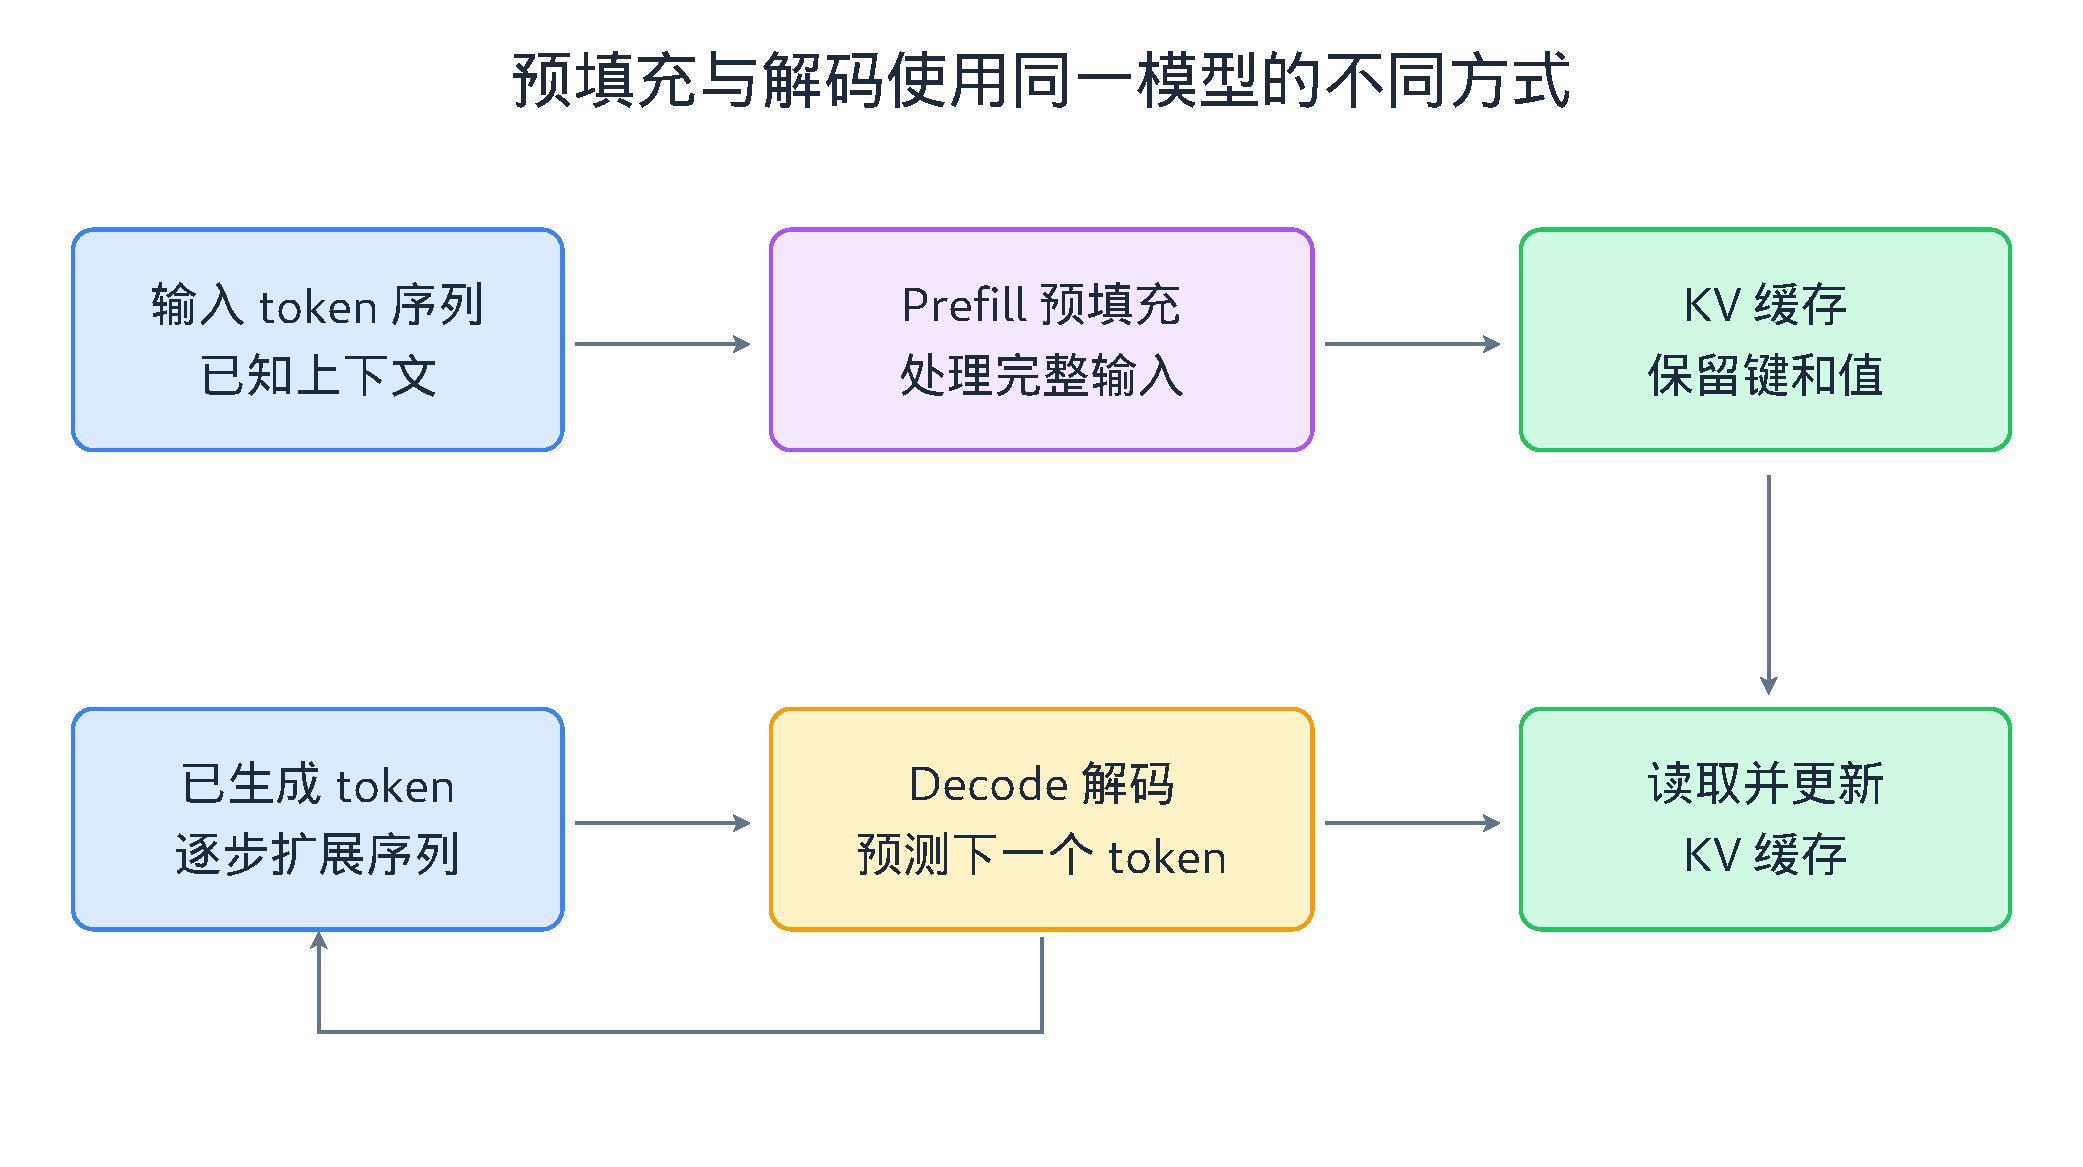
\includegraphics[width=\linewidth,height=.68\textheight,keepaspectratio]{assets/figure-04.pdf}
\caption{预填充与解码使用同一模型的不同方式，依据节目口述整理（00:40:55–00:50:57）}
\end{figure}
\begin{knowledgebox}{读图：大模型推理在忙什么：计算、搬运与等待}
图 4 分为上下两行。上行从左到右依次为：“输入 token 序列（已知上下文）”经箭头进入“Prefill 预填充（处理完整输入）”，再指向右侧的“KV 缓存（保留键和值）”。右侧“KV 缓存”有一条向下箭头指向下行的“读取并更新 KV 缓存”。下行左侧为“已生成 token（逐步扩展序列）”，向右进入“Decode 解码（预测下一个 token）”，再向右指向“读取并更新 KV 缓存”；同时从“Decode 解码”底部引出一条折返箭头指回左侧“已生成 token”，构成逐步扩展序列的循环回路。
\end{knowledgebox}
这一对比解释了为何单次并行处理完整输入的预填充更容易发挥算力吞吐，而需要循环预测下一个词元并反复读写键值缓存的解码阶段更容易受制于数据搬运。
\needspace{6\baselineskip}\subsection{本章小结}
本章拆解了大模型推理从接收提示词到持续生成词元的运行链路。推理过程的关键特征在于预填充（prefill）与解码（decode）两个阶段的差异：预填充阶段可对已知上下文做并行处理，主要消耗计算吞吐；而解码阶段采用自回归方式逐个生成词元，在小批量场景下需频繁从 HBM 读取模型权重与键值缓存（KV cache），容易受制于内存带宽与分布式互联延迟。为兼顾首词元时延（TTFT）、逐词元生成速度与尾延迟（tail latency），工程团队需在算子内核、编译器、推理服务框架运行时与集群调度四个层面协同优化，并借助经实机剖析校准的系统仿真来降低调优试错成本。
\needspace{8\baselineskip}\section{GPU 之外的路线与英伟达的系统优势}
上一章我们看到，大模型推理在预填充（prefill）与解码（decode）阶段呈现不同的负载特征：预填充适合大规模并行计算，而自回归解码阶段在小批量下容易受制于从高带宽内存（HBM）搬运权重与键值缓存（KV cache）的带宽开销。针对解码阶段的数据搬运瓶颈，芯片界尝试了哪些不同于传统 GPU 的硬件路线？本章将对比 Groq、Cerebras 与 SambaNova 三类数据流（dataflow）取向的加速器设计，探讨软件优化如何在给定条件下提升硬件利用率，并分析英伟达在芯片研发执行力与供应链协同上的优势。
\needspace{6\baselineskip}\subsection{Groq、Cerebras 与 SambaNova 各自改变什么}
传统 GPU 是一台高吞吐量流式处理器（high-throughput streaming machine），其大规模并行架构非常适合模型训练与推理预填充阶段。但在许多逐词元解码场景下，GPU 的计算与访存配比容易失衡：部分计算单元处于空闲（idle）等待状态，时间消耗在从片外 HBM 来回读取数据的过程上。软件社区为此开发了如 FlashAttention 等算法与算子优化，通过分块计算减少注意力层对高带宽显存的中间读写次数，尽可能让中间数据留在 GPU 片上高速存储中以贴近数据流计算的效果；但这类优化并不能消除全部权重搬运，也不会改变 GPU 的底层硬件形态，GPU 本身依然不是一台原生的片上数据流机器。

针对这一问题，由曾参与张量处理器（TPU）研发的成员创立并推出语言处理单元（LPU）的 Groq 采取了不同的架构取向。嘉宾在 00:51:16 处指出，Groq 的思路与他读博期间研究的众核数字信号处理器（Manycore DSP）相似，核心是采用基于片上静态随机存取存储器（SRAM）的数据流（dataflow）架构：尽量让工作负载的数据常驻在芯片片上存储中，通过软件确定性调度让计算任务像流水线一样依次流经不同的处理器核心（core），从而减少数据在片内与片外存储器之间的频繁往返（受单芯片 SRAM 容量限制，实际部署大模型时往往需要多芯片组成集群）。节目中还提到，围绕这类架构对解码阶段的加速作用，英伟达与 Groq 达成了相关交易与技术吸纳，而 AMD 也在其技术活动（Advancing AI）上展示了与 Cerebras 合作构建预填充与解码异构推理集群的方案。

与 Groq 在片上数据流思路上有相似之处的 Cerebras，同样强调利用大容量片上 SRAM 减少对外部 DRAM 或 HBM 的访问，但它在物理实现上走向了晶圆级（wafer-scale）集成（00:53:28）。传统造芯流程需要先将整片晶圆（wafer）切割成独立的裸片（die），分别封装后再在系统板卡级进行互联；而 Cerebras 直接将整片晶圆主体封装在一起，利用晶圆上预留的互连线完成核心间的片上连接，从而降低了部分跨芯片封装与板级走线的搬运开销。不过，晶圆级系统依然受单晶圆总存储容量与集群通信约束，且在工程上必须解决三大难题：
\begin{enumerate}
\item 垂直供电：整片晶圆面积大，无法像单颗小裸片那样仅靠四周边缘引脚供电，必须采用垂直供电方案；
\item 冷却散热（cooling）：大面积高功率晶圆对散热设计提出了很高要求；
\item 良率容错：制造出的晶圆不可避免存在局部缺陷，无法要求晶圆上每一部分都零缺陷，因此必须在片上互联中设计硬件路由机制，以绕过（bypass）损坏的单元。
\end{enumerate}
嘉宾评价称，虽然通过 3D 堆叠或高速互联也能实现扩展，但 Cerebras 探索的垂直供电等工程技术在数据中心芯片演进中具有前瞻性。

相比前两家高度侧重片上 SRAM 的设计，由嘉宾前甲骨文（Oracle）同事参与创立的 SambaNova 则采取了折中路线（00:58:02）。单纯依赖片上 SRAM 的架构面临明显的容量边界——当大模型参数规模很大时，若只靠片上存储就需要拼接更多数量的芯片。SambaNova 最初为兼顾 AI 计算与数据库负载而设计，它在采用可重构数据流架构并保留较大容量片上 SRAM 的同时，借助外部内存（嘉宾讨论中提及搭配 DDR 或 HBM 等外部 DRAM）来扩展单节点可容纳的模型容量，在片上流水效率与大模型容量适应性之间做工程折中。

\needspace{6\baselineskip}\subsection{软件怎样减少硬件浪费}
面对不同硬件架构与不同代际的制造工艺，主持人提出了一个工程问题：如果一方使用 2 纳米或 5 纳米芯片运行大模型，另一方只能使用 7 纳米或 12 纳米芯片，软件与基础设施层面的优化能追回多少差距（00:59:13）？肖志斌分析说，首先要明确软件无法改变芯片的物理工艺——软件不能把 7 纳米芯片变成 2 纳米，两者在同等性能下的晶体管功耗（机柜计算密度）以及串行输入输出接口（SerDes I/O）互联速率等物理边界依然存在。在他的工程经验估计中，7 纳米与 2 纳米在这些硬件指标上的差距大约在 2 到 3 倍的量级，同时考虑到片上 SRAM 在 5 纳米到 3 纳米阶段缩放趋缓，先进制程在访存密集型任务上的部分硬件收益还会有所折减。

在此基础上，嘉宾结合经验举例说明（00:59:45），针对尚未充分调优的系统，工程团队可以通过多层软件与系统手段来挖掘硬件潜力：
\begin{enumerate}
\item 预填充与解码分离（PD 分离）：将计算密集特征与访存受限特征不同的两个阶段分配到不同配比的计算资源上调度；
\item 量化与解码算法优化：引入低精度量化、推测解码（speculative decoding）以及多词元预测（multi-token prediction），减少单步数据搬运或一次预测多个词元；
\item 运行时调度与利用率提升：优化运行时（runtime）组织，例如嘉宾举例说，若能把某些场景下原本仅 30\% 至 50\% 的硬件利用率提升到 80\% 至 90\%，就能显著减少算力闲置。
\end{enumerate}
嘉宾据此认为，如果先进制程芯片上的软件没有做好优化，而成熟工艺团队把上述系统与软件优化做深做细，在特定推理任务上拿回约 2 到 3 倍的性能提升是可能的，从而有机会在实际产出上追近未充分优化的先进工艺硬件。

然而，软件优化并非落后制程的独占特权，这构成了算力竞争中的动态博弈。如果 7 纳米芯片通过深度优化能获得数倍加速，那么拥有 2 纳米芯片的团队在理论上同样可以应用相同的软件技术继续向前狂奔。但现实商业环境中的投入产出比（ROI）改变了这一平衡：拥有先进制程与充沛算力的团队，往往因为新一代芯片硬件迭代太快，不需要耗费高昂的人力与时间成本去抠极其细碎的系统级软硬件协同设计（co-design）；相反，工艺受限或硬件资源紧张的团队，则被倒逼着投入重兵去压榨每一分硬件潜能，这也解释了为何许多算力受限的团队反而能在系统软件层做出极具突破性的工程创新。

\needspace{6\baselineskip}\subsection{从 CUDA 到执行力：让算力像水电一样便宜}
既然大模型推理的工作负载正逐步收敛，且软件与专用架构有巨大施展空间，这是否意味着英伟达的护城河仅限于训练侧，而在推理侧将被众多初创公司瓜分？针对软件从业者常认为英伟达仅靠 CUDA 生态“躺赢”的印象，嘉宾从芯片架构师的视角给出了截然相反的判断：在软件行业眼中节奏似乎偏慢的英伟达，在芯片硬件行业却是执行力最强的公司，其架构演进的激进程度与研发速度堪比一家初创企业。

这种执行力体现在架构迭代与战略决策两个维度。在架构层面，当学术界与其他厂商还在围绕两倍稀疏化计算或特定优化方案撰写论文时，英伟达一旦从前沿模型研发团队拿到实际反馈（feedback），就会在后续 GPU 架构中快速将这些特性落地。在战略合作与交易层面，当看到数据流架构在解码阶段的互补价值或潜在竞争时，尽管外部架构与自身现有软件栈并不直接兼容，英伟达依然能迅速就 Groq 相关技术与团队做出交易决策（01:03:59）。嘉宾指出，这种创始人主导（founder-led）的快速决策机制，再加上其在台积电晶圆代工产能与 HBM 供应链上的大规模采购与深度协同优势，使得竞争对手即便设计出不错的推理架构，也会在产能获取与工程迭代速度上面临现实壁垒。

放眼整个 AI 行业，无论是编程工具因需求激增而出现服务中断，还是多模态与智能体基础设施（agent Infra）的扩展，都表明行业的核心诉求依然是增加有效算力并持续降低词元成本（token cost），让 AI 像自来水和电力等公用事业（utility）一样便宜易用。为此，半导体与系统工程师正从 KV 缓存管理、分布式推理、新型存储器件乃至光互联等多个方向持续攻关。不过，词元成本下降的速度同时受到物理世界建设周期的制约——嘉宾在 01:07:15 处举例指出，在美国新建电厂或输电电网项目往往需要 5 年以上的周期，而全球先进芯片的产出也受到晶圆厂扩产规律与 ASML 光刻机每年交付量的物理限制。

当物理世界的电力、晶圆与设备产能扩张无法一蹴而就时，软件与系统优化就成为打破算力僵局的关键抓手。当前由于大模型结构演进过快、异构硬件眼花缭乱，大量 GPU 集群实际上处于低效运行与特性闲置的状态。物理扩建的刚性限制，正倒逼行业从粗放堆卡转向极致的精细化调优。如何将资深芯片与系统架构师脑中的协同设计经验抽象成工具，让智能体（AI agent）能够自动、持续地完成跨模型与异构硬件的系统优化，从而把词元成本降到极致，正是下一阶段基础设施竞争的核心命题。

\begin{importantbox}{片上数据流（Dataflow）与晶圆级集成的工程权衡}
Groq、Cerebras 与 SambaNova 等非传统架构，均尝试通过数据流（dataflow）设计减少 GPU 频繁读写片外显存的开销，但在工程上各有取舍：
\begin{enumerate}
\item 片上容量与集群扩展：片上 SRAM 面积成本高且在 5nm 至 3nm 节点缩放趋缓，主要依赖片上 SRAM 的架构在面对超大模型时受单芯片容量限制，需依靠多芯片或多节点协同；SambaNova 则通过搭配外部内存换取更大的模型容量空间。
\item 晶圆级（Wafer-scale）工程约束：Cerebras 通过整片晶圆集成降低了部分跨芯片走线开销，但仍需面对晶圆容量边界与集群通信，并要在工程上解决垂直供电、大面积散热以及绕过（bypass）缺陷单元的容错路由问题。
\end{enumerate}
\end{importantbox}
\begin{knowledgebox}{教学算例：为什么软件优化能追回硬件制程代差}
软件优化不能改变芯片的物理制程、功耗上限或接口物理带宽，但可以改变硬件资源的实际有效利用率。为直观理解嘉宾在 00:59:45 处的经验讨论，可参考一个教学举例（仅作概念说明，非通用定律）：假设在相同的模型、输入序列长度、批大小与精度约束下，硬件 A 的理论峰值高于硬件 B，但硬件 A 仅运行未调优的基础配置，大量时间消耗在流水线等待与低效调度上；而团队在硬件 B 上通过 PD 分离、算子优化、推测解码与连续批处理调度，大幅减少了计算单元空闲时间。此时，硬件 B 在该特定任务上的实际有效吞吐可能追平甚至超过未充分调优的硬件 A。不过，一旦硬件 A 同样应用这些软件优化，物理制程与带宽的优势仍会体现出来。
\end{knowledgebox}
\begin{table}[H]\centering\small
\caption{节目讨论的四类 AI 加速器架构取向对比}
\begin{tabular}{>{\raggedright\arraybackslash}p{\dimexpr(\linewidth-6\tabcolsep)/3\relax}>{\raggedright\arraybackslash}p{\dimexpr(\linewidth-6\tabcolsep)/3\relax}>{\raggedright\arraybackslash}p{\dimexpr(\linewidth-6\tabcolsep)/3\relax}}
\toprule
架构/代表厂商 & 核心解决的问题 & 底层机制与工程取舍\\\midrule
传统 GPU（NVIDIA） & 大规模并行计算与通用生态兼容 & 高吞吐流式处理器配大容量 HBM；擅长预填充，但解码阶段易因片外内存搬运导致算力闲置。\\[4pt]
片上数据流 LPU（Groq） & 减少解码阶段片外内存频繁搬运 & 强调确定性调度与片上 SRAM 数据流，减少片外访存往返；单芯片容量有限，大模型需多芯片扩展。\\[4pt]
晶圆级数据流（Cerebras） & 跨芯片封装与板级互联的通信瓶颈 & 采用晶圆级集成减少部分跨裸片封装走线开销；需攻克垂直供电、大面积散热与缺陷单元绕过路由等工程问题。\\[4pt]
混合存储数据流（SambaNova） & 纯 SRAM 架构难以容纳超大模型 & 采用可重构数据流架构并结合片上 SRAM 与外部内存，在片上流水效率与大模型容量之间做折中。\\[4pt]
\bottomrule\end{tabular}\end{table}
面对解码阶段的数据搬运压力与大模型容量增长，不同芯片厂商选择了不同的架构切入点。图 5 汇总了节目所讨论的四类加速器路线及其各自侧重的系统改造位置。
\begin{figure}[H]\centering
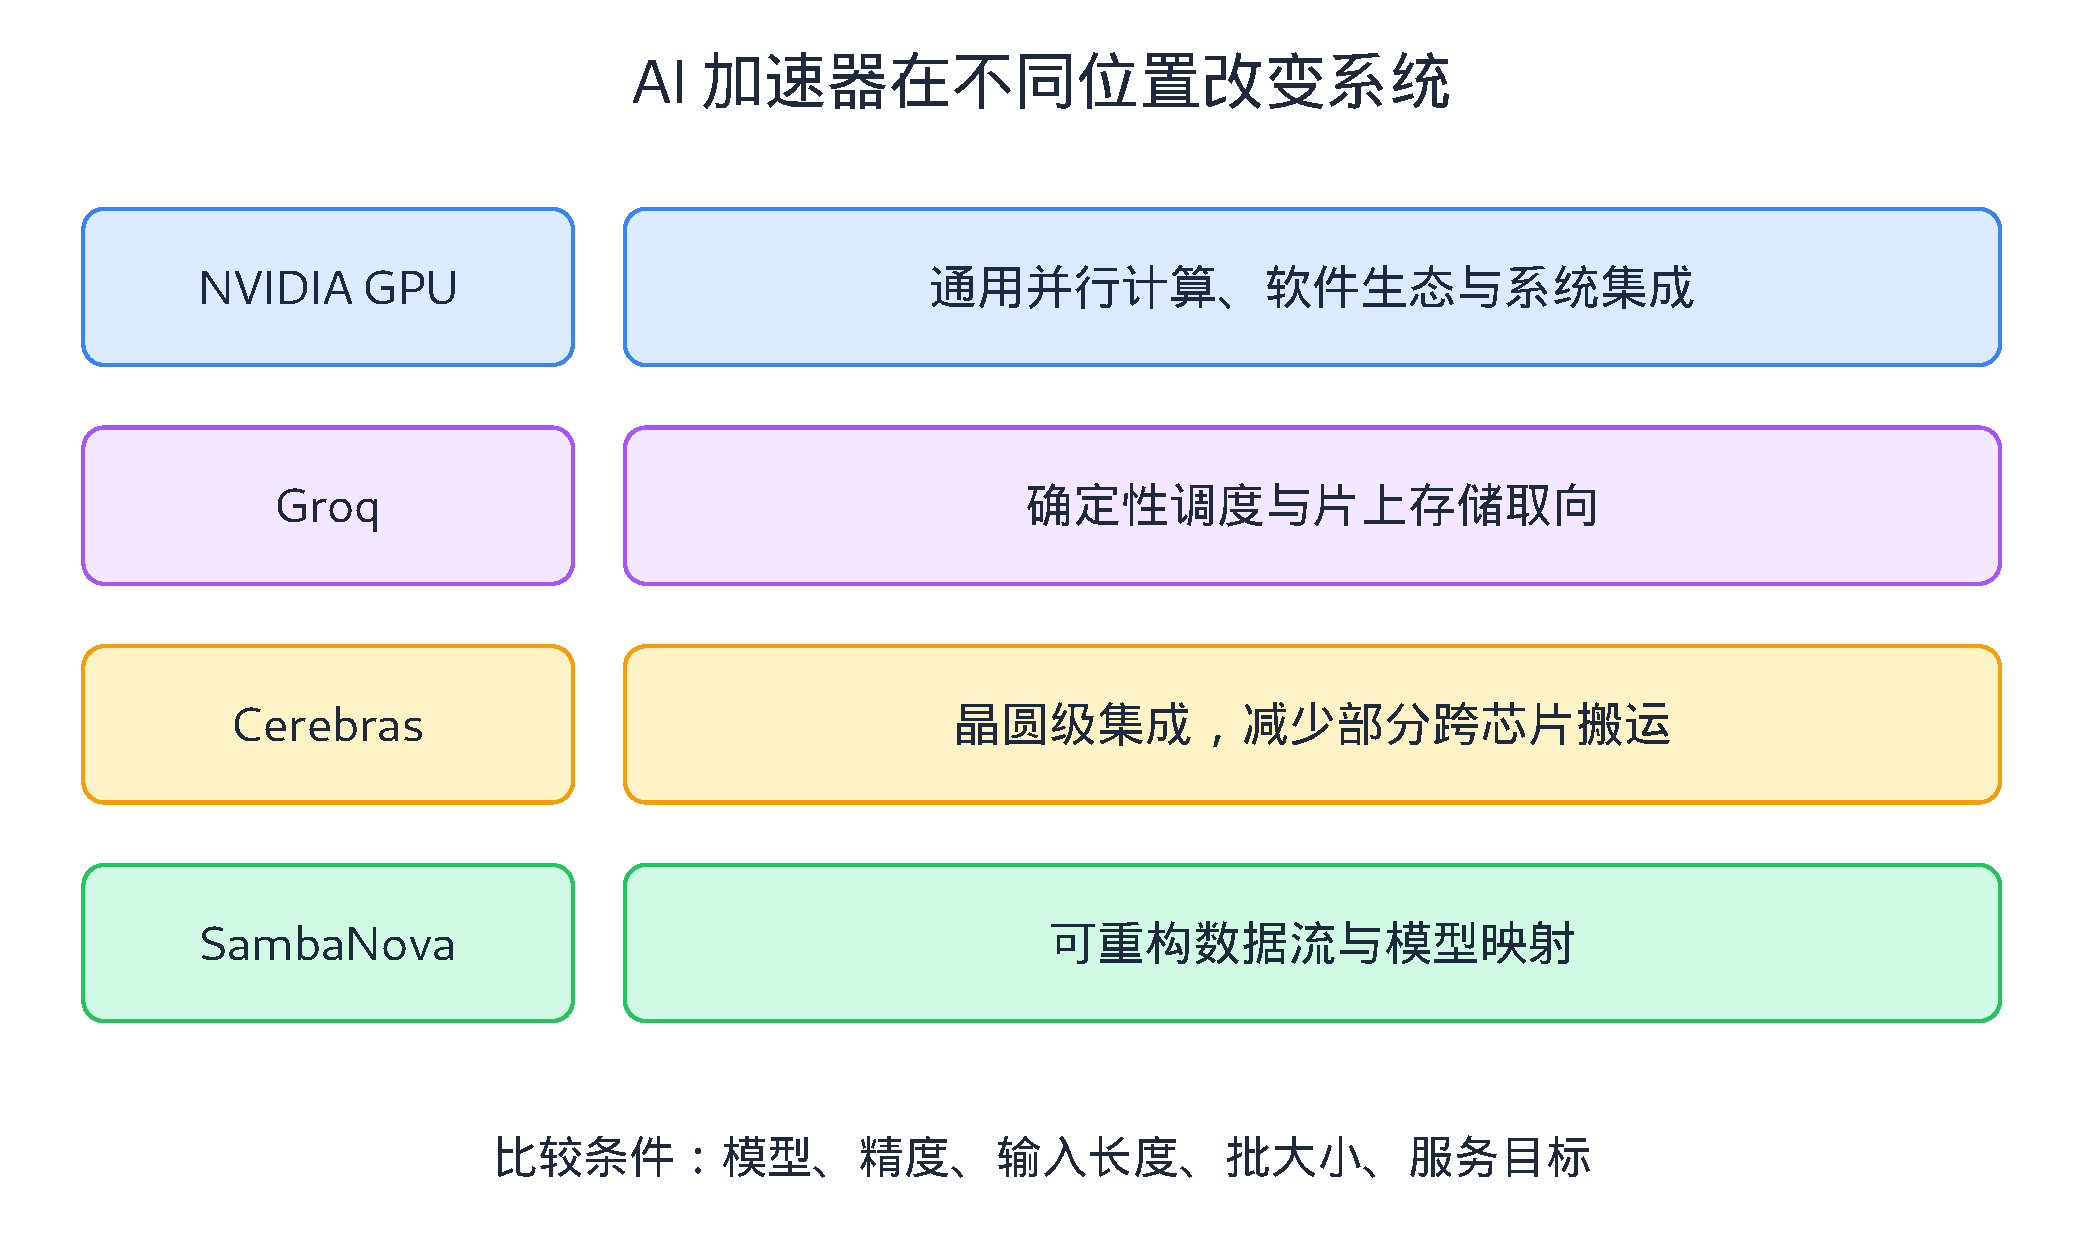
\includegraphics[width=\linewidth,height=.68\textheight,keepaspectratio]{assets/figure-05.pdf}
\caption{AI 加速器在不同位置改变系统，依据节目口述整理（00:50:57–01:09:54）}
\end{figure}
\begin{knowledgebox}{读图：GPU 之外的路线与英伟达的系统优势}
图 5 按四行并列展示了四类硬件路线，每行左侧为厂商或类别名称，右侧为其核心取向：第一行“NVIDIA GPU”对应“通用并行计算、软件生态与系统集成”；第二行“Groq”对应“确定性调度与片上存储取向”；第三行“Cerebras”对应“晶圆级集成，减少部分跨芯片搬运”；第四行“SambaNova”对应“可重构数据流与模型映射”。图底部明确标注：“比较条件：模型、精度、输入长度、批大小、服务目标”。
\end{knowledgebox}
图 5 说明这四条路线并非脱离条件的绝对性能排名，每种架构都在计算、片上存储、片间互联与模型映射之间做了不同取舍，必须在明确模型、精度、输入长度与批大小的前提下评估其系统收益。
\needspace{6\baselineskip}\subsection{本章小结}
本章对比了突破推理访存瓶颈的不同硬件取向与软件优化空间。Groq、Cerebras 与 SambaNova 分别从片上 SRAM 确定性数据流、晶圆级集成以及片上存储结合外部内存等方向改造数据流动方式，各有其适用场景与工程约束。在制程维度，软件虽无法改变 7 纳米与 2 纳米之间的物理功耗与接口带宽边界，但通过 PD 分离、量化、推测解码与运行时调度提升硬件利用率，可以在特定负载下显著缩小实际产出差距。与此同时，英伟达凭借软件生态、创始人主导的快速架构迭代与交易执行力，以及在台积电产能和 HBM 供应链上的协同优势，依然保持着强大的系统竞争力。面对电力与晶圆扩产等物理周期约束，通过软件与系统协同优化减少算力浪费，是持续降低词元成本的重要途径。
\needspace{8\baselineskip}\section{Oracle 到阿里：技术路线与职业选择}
在剖析了数据流架构、制程瓶颈与英伟达的系统级护城河之后，本章将视角拉回肖志斌个人的工业界实战轨迹。从甲骨文（Oracle）将数据库算子硬化进 SPARC 处理器的垂直整合，到阿里巴巴从零构建首代 AI 芯片的内部创业，这两段跨越中美巨头的经历不仅展现了一名资深芯片架构师如何通过软硬件协同设计（hardware-software co-design）解决实际系统瓶颈，也揭示了技术路线成败背后的生态规律与工程师的职业选择逻辑。
\needspace{6\baselineskip}\subsection{成熟组织与高速增长团队的工作方式}
博士毕业后，面对学术界与各类软硬件公司的选择，肖志斌在 01:10:11 处回忆，自己加入 Oracle 的核心动因是遇到了一个标杆性的软硬件协同设计新项目。在传统芯片行业中，架构师岗位通常由极资深的人士垄断，应届博士进入成熟大厂往往只能从验证或局部模块（block）做起，在既有流程上修修补补、逐级晋升。而当时 Oracle 刚刚以约 70 亿美元收购了拥有 SPARC 处理器、Solaris 操作系统、Java 与 MySQL 的太阳微系统公司（Sun Microsystems），正筹建名为“Software in Silicon”（软件功能硬件化）的新团队，试图将核心数据库操作直接固化到 CPU 硅片中。这种能够跨越硬件架构与底层软件、从头到尾观察系统全局的机会，构成了他早期职业选择的首要标准。

在 Oracle 的五年间，肖志斌从初级工程师一路成长为主任工程师（Principal Engineer）。他坦言当时公司内部存在一定的职级头衔膨胀（inflation），自己的 Principal 并非等同于英伟达等公司的顶级技术院士（Fellow），但快速的晋升确实源于承担了超越传统模块设计的架构职责。与被动接收规格说明书（spec）并转化为代码的普通工程师不同，他主动接手了数据压缩软硬件协同设计等极具挑战性的工作，并在更大职责范围（scope）内跨部门协调 CPU、操作系统与数据库运行时（runtime）资源，以直接的项目产出和影响力推动了职级跃升。

2017 年后，随着各大超大规模云服务商（hyperscaler）纷纷布局定制芯片，肖志斌选择加入阿里巴巴刚起步的芯片团队，负责第一代 AI 芯片（含光 800）的研发。与拥有全套成熟遗产的 Oracle 截然不同，互联网大厂造芯是一张白纸，入职之初甚至尚未明确具体要做哪类芯片。这种从 0 到 1 的“大公司内部创业”环境，迫使他的角色从单纯的芯片架构师向产品经理乃至商业决策者延展。

在高速增长的创始团队（founding team）中，肖志斌不仅要定义架构，还要承担大量传统上由芯片公司 CTO 或 CEO 负责的工作。实践经验表明，这一阶段的端到端建制包含四个关键步骤：1. 深入调研云端业务场景，核算不同工作负载的投资回报率（ROI，Return on Investment）与成本，判断业务能否沉淀为定制芯片；2. 引进芯片设计服务（design service）团队；3. 评估并采购第三方知识产权核（IP）；4. 与晶圆代工厂（foundry）谈判并签署首份合作协议。这种在模糊与不确定性中寻找确定性、拉通商业与技术全链条的历练，为他日后独立创业打下了坚实基础。

\needspace{6\baselineskip}\subsection{选择架构时怎样面对兼容与生态}
回到具体的工程技术机制，肖志斌在 Oracle 参与的数据库加速项目（DAX，数据分析加速器）旨在将协处理器（coprocessor）集成到 SPARC CPU 内部，使其与 CPU 共享全部内存带宽，从而加速内存型（in-memory）数据库的查询。整个加速器包含内存处理部分与查询处理器（query processor，即数据库查询加速引擎）两部分。面对系统设计中的权衡（trade-off），他在 01:14:22 处指出，当时团队做出的关键架构决策，是确立了“内存中存放压缩格式数据库、硬件读取并实时解压缩与计算、仅提取所需数据运算后写回内存”的技术路线，从而减少实际内存搬运量；他本人在其中负责 OZIP（Oracle ZIP，甲骨文压缩算法）相关的压缩架构算法与微架构设计。

将特定压缩算法硬化到芯片中存在一个工程风险：一旦业务数据类型发生改变，固定压缩方式的压缩效率可能明显下降。为了在硬件解压速度与数据适应性之间取得平衡，肖志斌团队在 OZIP 硬件实现中采用了一套基于查表（table lookup）的软硬件协同机制，其运行流程如下：
\begin{enumerate}
\item 数据库扫描与建表：考虑到数据库查询（query）场景下底层数据通常不会瞬间剧烈变动，软件先扫描一遍数据库，生成对应的压缩码字表（codeword table）；
\item 芯片预加载：在加速器开始运行查询任务前，将该码字表预加载（preload）到加速器的片上存储单元中；
\item 实时查表解压：当查询请求进入芯片后，硬件将读入的压缩数据与片上码字表进行查找匹配，实时解压缩出未压缩数据并送入后续的查询处理单元；
\item 更新码表适应变化：当数据库内容随时间变化后，可通过重新扫描数据库生成新的码字表并加载进芯片，以维持压缩与解压效率，从而降低了算法固化带来的风险。
\end{enumerate}

然而，尽管 Oracle 拥有从 SPARC 芯片设计、Solaris 操作系统、运行时调度到顶层数据库的极致垂直整合能力，这个在技术上极具创新性的项目最终却未能取得商业上的广泛成功，整个 SPARC 部门甚至在后期遭到裁撤。嘉宾强调，失败的核心症结不在于微观架构，而在于指令集兼容性与宏观软件生态的萎缩。

当时数据中心服务器的主流正在从 SPARC 加 Solaris 的小型机，转向 x86 架构加开源 Linux 的组合。SPARC 拥有独立的指令集，与 x86 二进制生态不兼容（尽管软件源码在投入工程改写与重编译后并非绝对不可迁移，但生态迁移成本很高），同时 Oracle 当时也没有将 Solaris 操作系统推向开源。这导致整個平台的生态不够繁荣，在 SPARC 上开发和维护上层应用的人越来越少，即便芯片内部与自家数据库配合紧密，整个技术栈在产业演进中还是逐渐失去市场。

\needspace{6\baselineskip}\subsection{开源、长期投入与团队执行}
SPARC 与 Solaris 的历史教训，自然引出了关于开源生态的深层探讨。肖志斌在 01:20:23 处从硬件、软件与大模型三个维度剖析了开源的产业逻辑。在硬件领域，诸如 SerDes（串行器/解串器）等绝大多数底层核心 IP 均依赖商业授权许可（license），像 RISC-V 这样开源的指令集架构实属罕见；但芯片造出来后必须依赖软件生态才能存活。回顾上一代互联网的繁荣，正是由 Google 发表的数篇分布式系统与数据库奠基论文，配合 x86 服务器、开源 Linux 操作系统以及开源大数据处理系统共同催生的。

而在当今的大模型开放权重（open model weights）浪潮中，开源与闭源的博弈则完全取决于参与者所处的竞争位置（position）：
\begin{itemize}
\item 行业领先者（先到者）：前期投入了巨额资金与算力训练前沿模型，若直接开源，将面临如何衡量投资回报率（ROI）并收回巨额沉没成本的商业难题；
\item 行业追赶者（后来者）：无论是企业还是国家层面，后来者往往倾向于通过开源来迅速做大自身生态、吸引全球开发者协同迭代，这也是追赶者打破垄断的常见策略；
\item 企业级应用方：若能将开源模型与框架改造得满足合规与安全性（safety）要求，企业不仅能显著降低调用成本，还能将其作为与闭源大模型厂商谈判的筹码（leverage），实现私有化部署（如部署开源智能体框架 OpenClaw）并牢牢把控自有数据；
\item 工程师个体：开源对个人而言是绝对的利好，工程师不仅能参与更复杂的工业级项目，其积累的技术能力与领域知识（knowledge）也具备极强的跨公司可迁移性（transferable）。
\end{itemize}

这种对技术生态与个人成长的洞察，也贯穿在肖志斌对青年工程师职业规划的建议中。节目讨论指出，年轻人在毕业初期固然可能面临解决签证身份、家庭稳定等现实考量，选择进入成熟大厂做按部就班的模块维护无可厚非；但若没有后顾之忧，应当尽量规避那些仅有光鲜头衔（title）、实则在陈旧流程上修修补补的岗位。趁年轻进入像新型 AI 基础设施（AI Infra）公司或大厂从 0 到 1 的创新项目，亲手把端到端的全流程跑通，才能真正建立起架构师的全局视野。

\begin{importantbox}{核心机制：OZIP 硬件加速中的码字表（Codeword Table）查表解压}
在 Oracle 的数据库加速器（DAX）中，为了减少内存读取量并配合查询处理器（query processor）高速运行，系统将数据库以压缩格式存放在内存中，并通过 OZIP 算法实现实时硬件解压缩。为降低数据类型变化导致压缩效率下降的风险，OZIP 采用了软硬件配合的查表机制：先扫描数据库生成码字表（codeword table），在运行前预加载（preload）至加速器片上存储；查询执行时，硬件对照码字表将压缩数据实时解压并送入后续查询计算；当数据特征改变时，可重新扫描数据库并更新码字表。这一机制在特定数据库查询负载下兼顾了带宽节省、硬件解压速度与数据适应性。
\end{importantbox}
\begin{knowledgebox}{工程经验：如何评估“从 0 到 1”的职业机会}
嘉宾结合自身在 Oracle 新建部门与阿里芯片创始团队的经历，总结了高成长性工程岗位的三个特征：第一，具备跨层视野，能够突破单一模块（如仅写 RTL 或仅做局部验证）的限制，接触到从底层硬件、运行时系统到上层业务应用的全链路协同（end-to-end scope）；第二，问题定义尚未完全固化，允许工程师参与从需求调研、商业 ROI 核算到技术规格制定的早期收敛过程；第三，技术栈尽可能拥抱主流开源生态，使个人在项目中沉淀的工程经验具备跨企业的长期可迁移性（transferability）。
\end{knowledgebox}
\begin{table}[H]\centering\small
\caption{Oracle 数据库加速项目与阿里首代 AI 芯片项目对比}
\begin{tabular}{>{\raggedright\arraybackslash}p{\dimexpr(\linewidth-6\tabcolsep)/3\relax}>{\raggedright\arraybackslash}p{\dimexpr(\linewidth-6\tabcolsep)/3\relax}>{\raggedright\arraybackslash}p{\dimexpr(\linewidth-6\tabcolsep)/3\relax}}
\toprule
对比维度 & Oracle（Software in Silicon） & 阿里巴巴（含光 800 创始团队）\\\midrule
组织与业务阶段 & 收购 Sun 后的成熟巨头，拥有全栈历史资产 & 互联网大厂内部从 0 到 1 创业，白纸起步\\[4pt]
核心技术任务 & 在 SPARC CPU 内集成 DAX 协处理器加速数据库查询 & 面向云端高并发业务定制首代专用 AI 推理芯片\\[4pt]
个人角色与边界 & 主任工程师，主导 OZIP 压缩微架构与软硬件协同 & 创始团队核心，兼顾架构定义、产品经理与供应链拓展\\[4pt]
生态与最终走向 & 指令集与 x86 不兼容且 Solaris 未开源，生态萎缩后裁撤 & 跑通云大厂定制芯片与外部 IP、代工厂协作的完整闭环\\[4pt]
\bottomrule\end{tabular}\end{table}
从 Oracle SPARC 数据库加速项目的经验教训到阿里云端芯片的从零立项可以看到，硬件架构的成败从不只由单一性能指标决定。图 6 概括了具体产品与团队在做技术取舍时必须同时面对的四重约束。
\begin{figure}[H]\centering
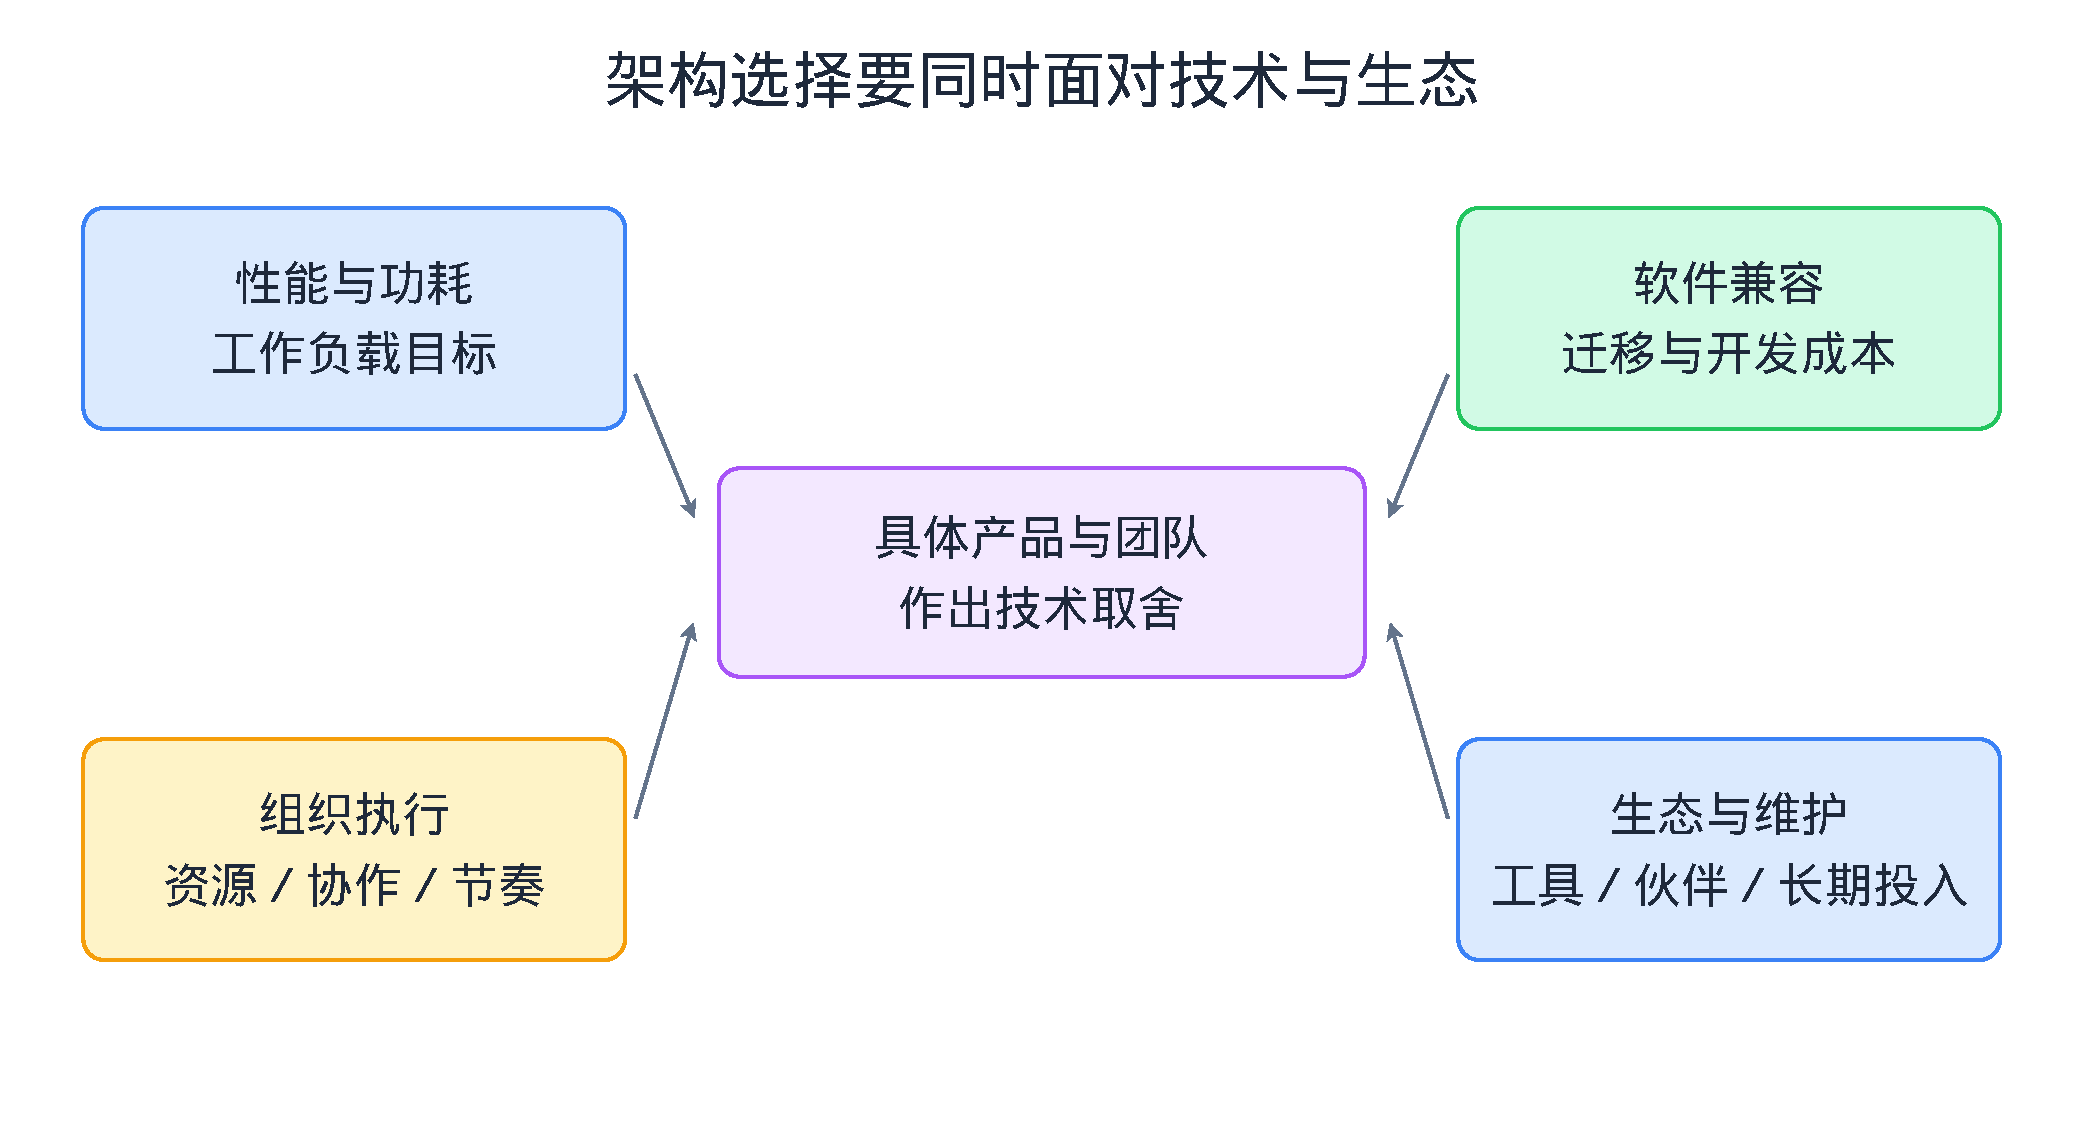
\includegraphics[width=\linewidth,height=.68\textheight,keepaspectratio]{assets/figure-06.pdf}
\caption{架构选择要同时面对技术与生态，依据节目口述整理（01:09:54–01:29:21）}
\end{figure}
\begin{knowledgebox}{读图：Oracle 到阿里：技术路线与职业选择}
图 6 中心位置是一个矩形框“具体产品与团队（作出技术取舍）”，四周分布着四个约束框，并分别以箭头指向中心框：左上角为“性能与功耗（工作负载目标）”，右上角为“软件兼容（迁移与开发成本）”，左下角为“组织执行（资源／协作／节奏）”，右下角为“生态与维护（工具／伙伴／长期投入）”。四支向内汇聚的箭头表明，中间的产品架构决策受到这四个维度的共同制约。
\end{knowledgebox}
这解释了为什么即便芯片内部微架构设计精巧，一旦软件兼容性不足或外部生态萎缩，产品依然难以持续；对工程师个人而言，评估职业机会同样需要综合审视这些真实工作维度。
\needspace{6\baselineskip}\subsection{本章小结}
本章回顾了肖志斌从 Oracle 到阿里巴巴的两段职业经历。在 Oracle 期间，他参与“Software in Silicon”项目，在 SPARC 处理器内嵌的 DAX 数据库加速器中负责 OZIP 压缩微架构设计，利用预加载码字表（codeword table）的查表机制实现了压缩数据库的实时硬件解压与查询配合；但受制于 SPARC 与 x86 生态的差异以及 Solaris 未开源导致的开发者流失，该项目最终随部门裁撤而落幕，体现出软件生态对硬件技术路线的重要影响。随后在阿里从 0 到 1 参与筹建第一代 AI 芯片含光 800 的经历，则让他从芯片架构师拓展到业务 ROI 评估、设计服务引入、IP 采购与代工厂合作等全链路工作，为后续创业打下了基础。
\needspace{8\baselineskip}\section{ZFlow.AI：用虚拟仿真寻找真实收益}
在甲骨文和阿里巴巴完成了从底层微架构创新到全链路芯片立项的历练后，肖志斌进一步跨入创业赛道，先后参与了两家初创企业。从上一家稀疏化 AI 芯片公司的 Chief Architect（首席架构师），到如今亲自担任系统优化公司 ZFlow.AI 的 CEO（首席执行官），他不仅将芯片研发中最核心的架构仿真方法论迁移到了软件基础设施领域，更在工程落地与商业化探索中直面 AI 算力调优的真实痛点。
\needspace{6\baselineskip}\subsection{从架构师到 CEO：找到客户问题}
离开阿里巴巴后，肖志斌先后参与了两家创业公司。在上一家专注于稀疏化 AI 芯片的初创企业中，他担任首席架构师（Chief Architect），工作重心延续了芯片架构设计，同时进一步向系统软件延伸，参与了运行时系统（runtime）团队的建设，并将此前在阿里积累的寻找合作伙伴与供应链对接的经验带入团队。而在创办 ZFlow.AI 时，他选择出任 CEO。嘉宾解释（01:29:39），这一角色转换的原因在于：卖芯片与卖 AI 基础设施（AI Infra）软件面临不同的商业模式问题。

在肖志斌看来，传统芯片公司的市场进入策略（go to market）路径相对明确：如果团队定义好架构并在两年后造出有竞争力的芯片，后续商业化主要是销售芯片、板卡及配套软件服务（当然，芯片本身能否研发成功并在两三年后依然具备市场竞争力，仍面临很高的工程与竞争风险）。相比之下，AI Infra 软件领域变化很快，即便团队做出了优化工具与产品，究竟该如何定价、提供何种交付形态——是做咨询（consulting）、技术服务（service），还是采用订阅制（subscription）——都需要在市场上摸索。为了将技术创新与商业模式探索结合起来，他决定亲自担任 CEO。

担任 CEO 后，他在继续跟进产品定义与核心技术细节的同时，将大部分时间投入到了商务拓展（BD）中。他的日常工作包括寻找合作伙伴、与潜在客户交流、签署谅解备忘录（MOU，用于确立合作意向，并不直接等同于已实现的商业收入）以及共同探讨商业模式。在资金使用与融资节奏上，团队保持着较低的资金消耗率（burn rate）。肖志斌倾向于先通过客户沟通把业务逻辑讲通，做出实际价值并获得付费用户，再集中短期时间窗口推进融资，尽量避免长期分散做业务的精力。

ZFlow.AI 的核心团队规模不大，仅有数人，主要由肖志斌的博士师弟、前同事等有过合作经历的行业老兵组成。团队成员背景涵盖从 0 到 1 搭建过云厂商异构 GPU 云服务（GPU cloud）的架构师，以及在芯片会议 Hot Chips 发表过论文、长期从事仿真器（simulator）研发的工程师。嘉宾谈到，面对如今复杂的大模型与异构集群，刚毕业且缺乏工业界或开源社区历练的新人很难直接上手底层系统调优；而他们这批兼具软硬件协同设计与云端部署经验的架构师，正是在用工具化的方法解决自己过去遇到的工程痛点。

\needspace{6\baselineskip}\subsection{系统建模、虚拟试验与实机校准}
为了具体说明虚拟仿真如何辅助实机调优，肖志斌分享了团队在英伟达 B300 硬件上优化 DeepSeek V4 模型的一次项目实践（01:34:28）。在模型发布早期（Day Zero 阶段），ZFlow.AI 与一家提供 GPU 资源的新型云服务商（neocloud）合作，在 8 卡 B300 环境上开展推理调优。面对这一模型，团队首先需要做出配置决策：在 8 张 GPU 卡中，是采用混合部署，还是采用 PD 分离（预填充 prefill 与解码 decode 分离）？如果采用分离方案，分别应分配几张卡做 prefill、几张卡做 decode？

如果不借助仿真工具，工程师往往只能占用真实 GPU 反复试错。而在该案例中，ZFlow.AI 的工作流包含四个相互配合的步骤：
\begin{enumerate}
\item 架构建模与虚拟仿真：利用仿真器对不同卡数配比和部署策略进行设计空间探索（design exploration），在不占用大量实机算力的情况下筛选出有潜力的候选配置（configuration）；
\item 实机自动性能分析（Auto-profiling）：在真实硬件上采集底层算子执行开销与动态运行数据；
\item 仿真模型校准（Calibration）：将实机采集的剖析数据输入回仿真器，修正仿真模型的参数；
\item 运行时配置与工程调优：将筛选出的配置应用到开源推理服务运行时框架（serving runtime）中，并投入工程精力调稳高并发下的框架运行状态。
\end{enumerate}
据嘉宾在节目中报告，在该 8 卡 B300 实机测试案例中，调优后的峰值吞吐量约为对照配置的 1.5 倍，尾延迟（tail latency）也有约 2 到 3 倍的改善（01:34:13）。

在谈到这套仿真模型与实机运行结果的吻合程度时，肖志斌介绍了团队在 DeepSeek 模型上的评估情况（01:38:54）：据其报告，仿真器在 prefill 阶段的仿真精度可超过 90\%，在 decode 阶段约为 80\% 到 90\%（节目口述未展开该精度指标的具体统计定义，实际误差会随模型结构与动态负载特征而变化）。为什么 decode 阶段更难仿真？嘉宾解释，这是因为实际运行中包含许多难以仅靠静态预编译准确预测的动态行为，主要包括：
\begin{enumerate}
\item 动态批处理与并发（Concurrency）：用户请求到达的时间与长度随机变化，导致批处理（batching）状态时刻改变；
\item 混合专家路由（MoE 调度）：在混合专家模型（MoE）中，不同的输入数据分布会触发不同的专家（expert）激活与路由路径；
\item 分布式网络通信：跨卡与跨机互联涉及网络拓扑结构（topology）、交换机（switch）转发、路由策略以及拥塞控制算法。
\end{enumerate}
如果对每一个网络包和动态细节都做逐周期模拟，仿真速度会过慢；因此需要依靠架构师经验对系统做合理抽象，使其达到足以指导调优（good enough）的程度，同时通过实机剖析（profiling）数据持续校准仿真模型。

从工具定位来看，肖志斌将这套系统比作面向芯片与数据中心架构探索的架构级 EDA 工具，同时也希望将其作为虚拟后端（Virtual backend）提供给开源推理服务生态使用。正如黄仁勋在英伟达 GTC 大会上提出 DSX Air（AI token factory simulator，AI 词元工厂仿真器）的概念一样，AI 硬件与系统软件的复杂性使得纯靠实机盲调成本高昂。肖志斌表示，不同于芯片厂商主要面向自家硬件的内部仿真工具，ZFlow.AI 的目标是构建一个中立（neutral）的跨架构平台，希望支持将英伟达、AMD 或其他厂商的硬件组合在一起做联合仿真与优化探索，帮助用户在缺乏充足 GPU 或采购部署前评估不同系统方案。

\needspace{6\baselineskip}\subsection{把优化结果交给客户：价值与商业模式}
除了模型推理服务（serving）层面的调优，ZFlow.AI 还将自动调优思路延伸到了智能体层面（agent level），开发了面向开源智能体框架 OpenClaw 的自动调优工具（OpenClaw AutoTuner）以及内存管理器（memory manager，01:42:25）。肖志斌解释，这对应于两个不同层次的优化：模型服务层重在优化推理框架与硬件配置，而智能体层的调优则根据用户的交互行为特征，决定如何选择模型、如何配置智能体的记忆或内存分配，从而减少人工逐案调参的工作量（在真实业务中，模型选择与路由除考虑成本外，还需兼顾任务完成质量与响应时延；同时智能体层面的记忆与上下文管理也不同于底层 GPU 硬件的显存物理分配）。

在技术机制上，这种跨层级的 AI 自动调优与肖志斌早年在甲骨文研究的数据库 query optimizer（查询优化器）有着深刻的传承关系。数据库的查询优化同样需要决定计算任务放在 CPU 还是加速器上执行、内存如何 allocate（分配），甚至因为存在大量 data dependent（数据依赖）的随机行为而比以矩阵运算为主的 AI 模型更加复杂。然而，随着如今的大模型引入 MoE 动态路由、动态批处理以及复杂的智能体工作流，AI 计算正呈现出越来越强的随机性与动态性，这使得昔日数据库优化器的算法思想在 AI 时代焕发了新的生命力。

尽管技术逻辑一脉相承，但回顾历史，独立做数据库优化器或加速器的初创公司却鲜有商业上的巨大成功。肖志斌清醒地剖析了其中的原因：一方面，业务形态变化极快，底层软硬件技术栈过深，纯做上层优化器的软件团队很难跟上底层硬件的迭代；另一方面，数据库原厂往往自带优化器，使得第三方工具极难界定清晰的商业边界。这一历史镜鉴直接映射到了当下的 AI Infra 创业环境中（01:45:37）。

基于这一历史经验，肖志斌提出了他对当前 AI Infra 创业环境的一个判断：在他看来，一家纯粹只做第三方软件优化的公司很难单独站稳位置，往往需要在两端中至少靠拢一头：
\begin{enumerate}
\item 绑定核心客户：拥有信任团队、愿意将业务交给团队持续调优的客户；
\item 结合底层算力资源：自身掌握或紧密结合 GPU 算力资源（正如市面上不少 AI Infra 公司实际上带有 GPU 资源服务属性）。
\end{enumerate}
节目中，主持人将这种构建虚拟后端与抽象层的尝试类比为早年做虚拟机的 VMware，认为若能跑通商业模式将具备很大潜力；肖志斌也表示，团队正通过“中立虚拟仿真平台 + 架构师团队 + 自动调优工具”的组合，在解决技术与商业化双重挑战的过程中稳步探索。

\begin{importantbox}{核心机制：为什么虚拟仿真必须配合实机校准（Calibration）？}
纯静态仿真只能在预编译（precompile）阶段根据计算图和硬件参数做初步估算。但在真实的分布式大模型推理中，用户请求的随机并发到达（batching 动态性）、MoE 模型中随输入数据分布变化的专家路由（expert 调度），以及交换机拓扑与拥塞控制，都是运行期（runtime）动态变化的行为，仿真也不是对每个词元做真实数值计算。因此，ZFlow.AI 通过在真实硬件上运行自动性能分析（Auto-profiling），采集算子启动开销与运行分布特征并反馈给仿真器做参数校准（calibrate）。在嘉宾报告的 DeepSeek 测试中，经过校准的仿真在 prefill 与 decode 阶段分别达到了 90\% 以上和 80\%–90\% 的吻合度，从而能够辅助筛选有潜力的部署配置。
\end{importantbox}
\begin{knowledgebox}{经验洞察：数据库查询优化器与 AI 系统自动调优的异同}
在传统关系型数据库中，查询优化器（Query Optimizer）负责分析 SQL 语句并决定最优的执行计划与内存分配；由于涉及大量数据依赖（data dependent）的条件分支，其运行轨迹高度随机。相比之下，早期的深度学习模型以固定的稠密矩阵运算为主，行为高度可预测。但随着混合专家模型（MoE）、连续批处理（continuous batching）以及多步智能体框架（如 OpenClaw）的普及，AI 推理负载正变得越来越像数据库查询，充满了运行期动态路由与异构存储调度。这也使得借鉴数据库优化器思想、构建端到端的 AI 自动调优器（AutoTuner）成为必然趋势。
\end{knowledgebox}
\begin{table}[H]\centering\small
\caption{ZFlow.AI 系统优化体系的三个核心层级与机制对比}
\begin{tabular}{>{\raggedright\arraybackslash}p{\dimexpr(\linewidth-6\tabcolsep)/3\relax}>{\raggedright\arraybackslash}p{\dimexpr(\linewidth-6\tabcolsep)/3\relax}>{\raggedright\arraybackslash}p{\dimexpr(\linewidth-6\tabcolsep)/3\relax}}
\toprule
优化层级与组件 & 解决的核心问题 & 关键技术机制与实效\\\midrule
架构级虚拟仿真器（Simulator） & 缺乏真实 GPU 资源时的硬件选型与集群配比探索 & 对计算、存储与网络拓扑做架构级抽象，目标是支持跨厂商异构硬件的中立仿真与虚拟后端测试\\[4pt]
推理服务层调优（Serving AutoTune） & 分布式推理中吞吐量受限与长尾延迟（Tail Latency）过高 & 结合仿真筛选候选方案与实机 Profiling 校准，辅助决策 PD 分离配比与并行配置（嘉宾报告 8 卡 B300 测试案例中峰值吞吐约为对照的 1.5 倍，尾延迟改善约 2–3 倍）\\[4pt]
智能体与内存层调优（OpenClaw AutoTuner \& Memory Manager） & 复杂 Agent 工作流下的模型选择与记忆/内存配置繁琐 & 根据用户行为特征，在智能体层面自动优化模型选择与 memory 相关配置，配合底层推理服务调优\\[4pt]
\bottomrule\end{tabular}\end{table}
由于真实推理集群中存在并发批处理、MoE 专家路由和网络通信等动态行为，纯静态仿真无法单独保证预测精度。图 7 展示了 ZFlow.AI 将虚拟试验与实机测量相结合的闭环校准流程。
\begin{figure}[H]\centering
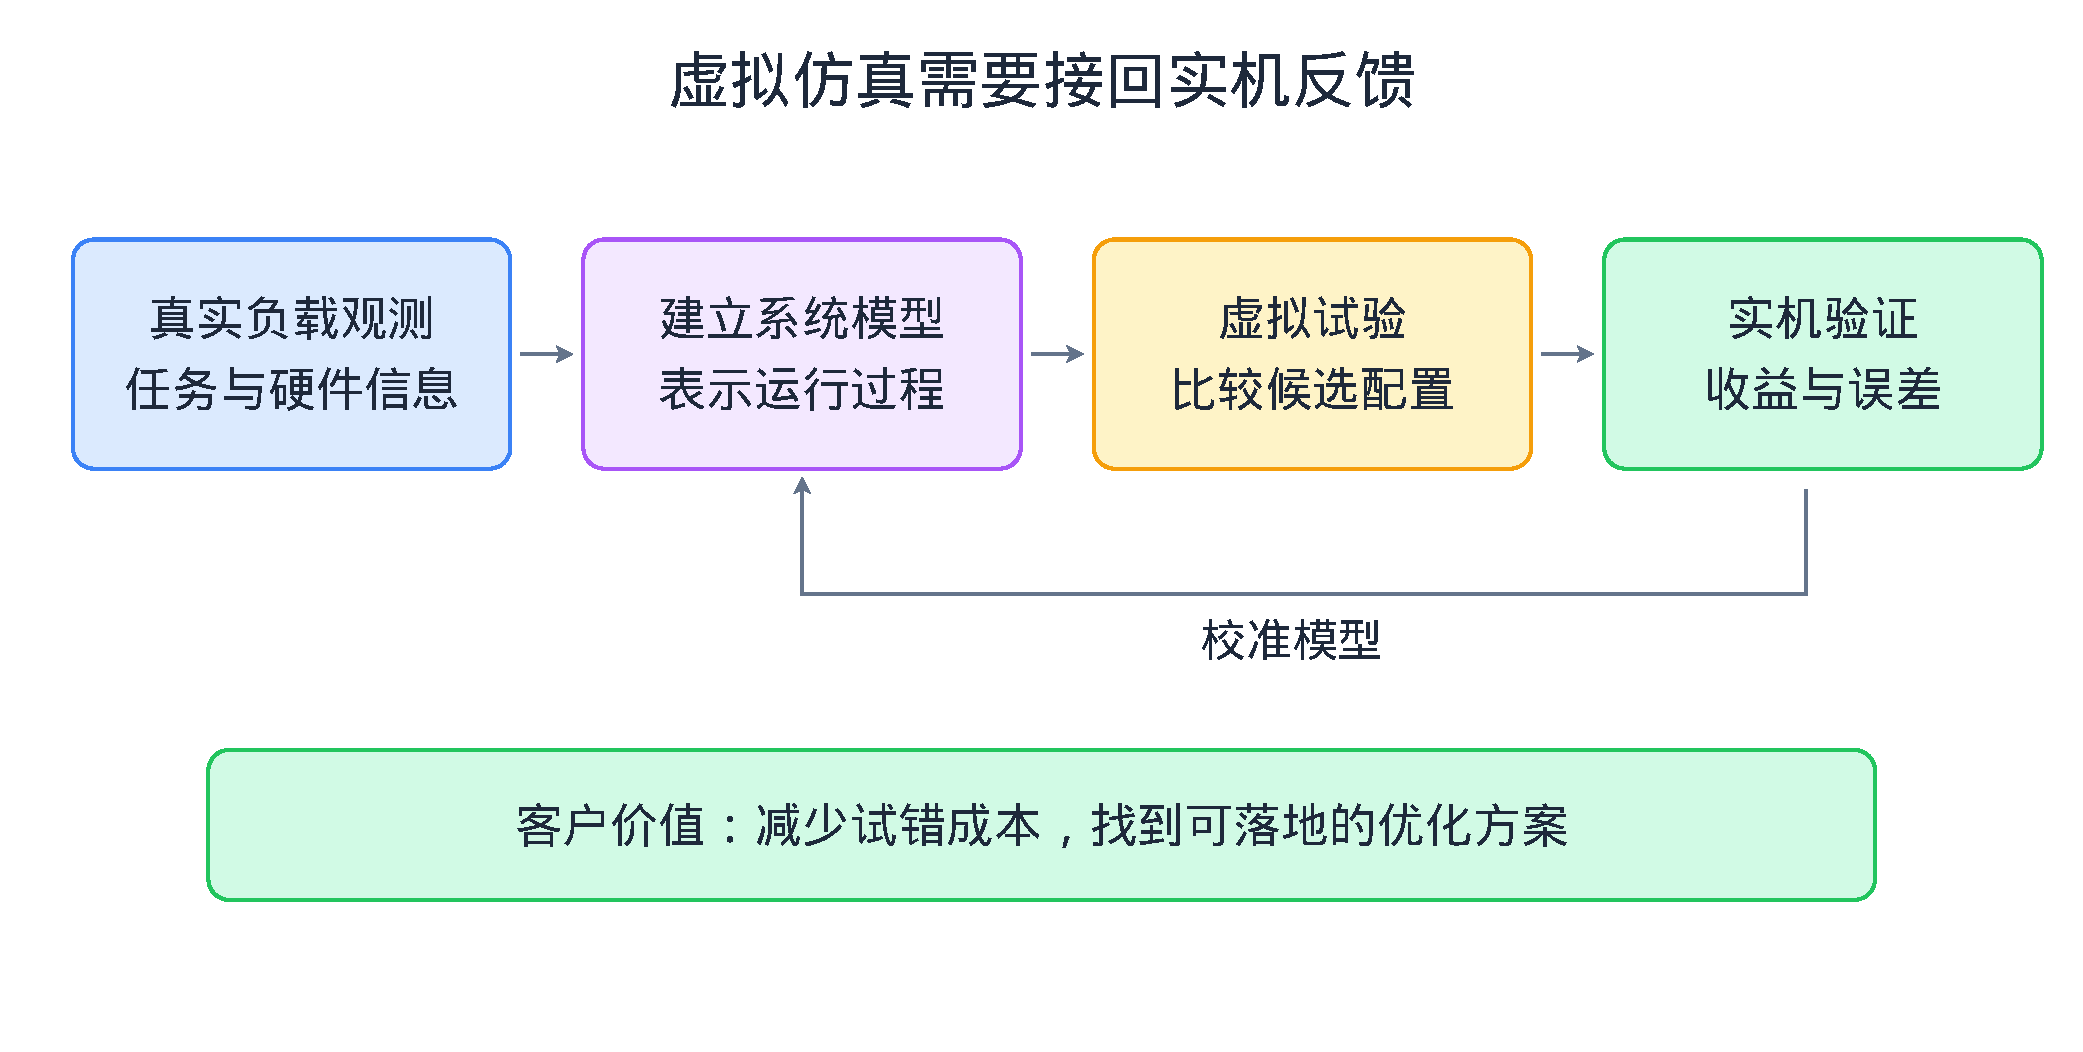
\includegraphics[width=\linewidth,height=.68\textheight,keepaspectratio]{assets/figure-07.pdf}
\caption{虚拟仿真需要接回实机反馈，依据节目口述整理（01:29:21–01:50:46）}
\end{figure}
\begin{knowledgebox}{读图：ZFlow.AI：用虚拟仿真寻找真实收益}
图 7 上方从左至右依次排列四个步骤框，以水平箭头顺次相连：“真实负载观测（任务与硬件信息）”\ensuremath{\rightarrow}“建立系统模型（表示运行过程）”\ensuremath{\rightarrow}“虚拟试验（比较候选配置）”\ensuremath{\rightarrow}“实机验证（收益与误差）”。从最右侧的“实机验证”底部引出一条向左折返的反馈箭头，标注为“校准模型”，直接指回第二个框“建立系统模型”。图最下方设有一个长框，写明“客户价值：减少试错成本，找到可落地的优化方案”。
\end{knowledgebox}
图 7 的反馈回路表明，虚拟仿真用于缩小候选空间、减少实机盲目试错，而实机验证测得的收益与误差又反过来校准系统模型，两者结合才能产出可靠的部署配置。
\needspace{6\baselineskip}\subsection{本章小结}
本章介绍了肖志斌创办 ZFlow.AI 并从首席架构师转向 CEO 的实践与思考。面对 AI Infra 软件在定价与交付形态上的不确定性，他通过高频的客户沟通与较低的资金消耗率探索商业模式。在技术上，ZFlow.AI 将芯片设计中的架构仿真方法引入数据中心调优，致力于打造跨厂商的中立虚拟后端；通过“虚拟仿真筛选候选配置 + 实机自动 Profiling 校准模型”的闭环，应对并发批处理、MoE 专家路由与网络通信带来的动态性，并在嘉宾报告的 8 卡 B300 运行 DeepSeek V4 案例中取得了峰值吞吐约 1.5 倍、尾延迟改善约 2–3 倍的实测效果。同时，团队将自动调优延伸至 OpenClaw 智能体层面，并结合数据库优化器的历史经验，提出 AI Infra 公司需贴近核心客户或算力资源的商业判断。
\needspace{8\baselineskip}\section{AI 时代的工程师：基础、工具与长期选择}
在第七章中，我们看到 ZFlow.AI 如何将芯片架构仿真的思维引入数据中心，通过虚拟后端与实机校准来解决多卡集群与智能体调优的复杂难题。正如节目讨论所指出的，这类底层系统极其复杂，刚毕业且缺乏工业界或开源社区深度历练的新人很难直接上手，而老一代架构师脑海中的实战资产又往往源自真金白银的“试错”。当 AI 与 agent（智能体）接管越来越多的日常开发工作，新一代工程师究竟该如何获取经验？作为全书的尾声，本章将顺着访谈最后的探讨，从半导体与互联网行业的资本结构变迁切入，解析工程师薪酬背后的供需逻辑，并探讨在 AI 原生时代学习计算机的价值与长期职业选择。
\needspace{6\baselineskip}\subsection{薪资变化背后的供需结构}
在硅谷的科技产业版图中，长期存在着一个令外界颇感意外的薪酬倒挂现象：同样身处技术前沿，传统芯片工程师的平均薪资水平，往往明显低于互联网大厂的软件工程师。嘉宾结合自己二十余年的从业经历回忆道，过去身边不少半导体行业的朋友为了更高的 pay（薪酬），纷纷转行去做软件开发，而像他们这样二十年如一日留在芯片行业深耕的“战斗老兵”反而成了少数。

为什么技术门槛高、试错代价大的芯片行业，给普通工程师开出的薪资往往不如互联网软件行业？在 01:50:54 处，嘉宾从企业成本结构的角度给出了他的解释。芯片设计公司的大量资金消耗在前期硬件与研发投入上，主要包括：
\begin{enumerate}
\item 硬件与仿真设备等固定资产投资；
\item 动辄数千万乃至上亿美元的流片（tape-out）费用；
\item 商业 EDA 软件的授权许可（license）费用；
\item 第三方硬件 IP 的采购许可费用。
\end{enumerate}
嘉宾认为，在这样的成本结构下，除了少数负责定义系统的顶尖架构师外，大部分普通芯片工程师日常主要是使用成熟的 EDA 工具完成模块开发与验证，人力支出在公司总投入中的占比相对不如纯软件公司突出（需注意，企业成本结构只是影响薪酬的因素之一，不能直接由成本占比简单推导单个岗位的具体工资）。

相比之下，在没有大规模建设 GPU 集群与 AI 基础设施之前的传统互联网时期，软件公司的成本结构有所不同。虽然互联网企业同样有服务器与数据中心支出，但无需承担晶圆流片或昂贵 EDA 授权等芯片研发开支，研发投入的很大比例直接用于招揽软件工程师。一旦核心软件代码开发完成，软件本身复制的边际成本很低，更容易扩展（scale）服务海量用户，因此软件工程人力在当时享有较高的薪酬溢价。

然而，进入大模型时代后，这种资本支出结构正在发生变化。嘉宾指出，如今的超大规模云服务商（hyperscaler）和互联网大厂在资本结构上变得越来越像半导体公司——庞大的数据中心、GPU 集群与电力基建，使得资本性支出（CAPEX，用于购置长期硬件与基础设施等固定资产的支出）成为了企业最大的投资项。与此同时，企业获取收入（revenue）的成本与底层硬件 CAPEX 呈现出更强的正比例关系，难以再单纯依靠人力编写软件实现低硬件成本的扩张。嘉宾认为，这种投资重心向硬件基础设施的转移，正在改变科技行业对普通软件工程岗位的供需与定价。

\needspace{6\baselineskip}\subsection{学习计算机的价值如何变化}
随着企业资本向硬件基建倾斜，大模型研发与软件工程内部的岗位分工也在经历剧烈重构。节目讨论指出，当大模型从 pre-training（预训练）、mid-training（中期训练）到 RL（强化学习）的整套训练链路搭建成熟后，常规环节中单个人力的不可替代性正在下降，甚至出现了由大模型辅助和指挥初级人员去执行标准化训练操作的趋势。

为了说明这一转变，嘉宾在 01:52:45 处提出了一个类比：\textbf{在未来的软件工业中，大模型就像半导体行业里的 EDA 工具，而许多普通软件工程师正在变成“使用 EDA 工具的人”}。在他看来，正如芯片行业里少数顶尖架构师能够维持丰厚的收入与回报，AI 行业里媒体报道的极高薪酬实际上也只集中在极少数核心人才身上；随着行业进入平稳期，主要依赖 AI 工具完成常规开发的普通软件工程师，其薪资结构可能会像传统半导体工程师那样发生变化。

面对这样的行业变化，高中生和年轻学子在今天还有必要学习计算机科学、或者从事芯片研发吗？在 01:54:14 处，嘉宾给出了肯定的回答：“还需要，人人都要变成架构师。”他解释说，工具变强并不意味着底层知识不再重要；相反，工程师需要具备上下拉通的视野，用工具帮自己实现复杂的工程目标，这对人的综合能力提出了更高要求。

因此，学习计算机的价值不再是死记硬背某种语法或充当熟练的代码翻译机，而是去掌握计算机底层的运行机理。在此基础上，年轻工程师还需要主动拓宽边界：既要向下扎根理解硬件与系统的底层逻辑，又要向上延伸去学习商业模式（business），搞清楚技术如何转化为真实的商业价值。

\needspace{6\baselineskip}\subsection{在 AI 原生工作方式中培养判断}
如果说未来的核心竞争力在于“人人都要成为架构师”，那么在日常的 AI-native（AI 原生）工作方式中，工程师究竟应该刻意培养哪些无法被工具轻易替代的能力？嘉宾根据实践经验指出，除了扎实的底层基础与商业认知外，最关键的是在实践中磨炼出属于自己的 taste（判断品味）与 know-how（实践诀窍）。面对复杂的系统权衡，能够穿透表面现象识别出真正的性能瓶颈与需求边界，这种架构师式的思维与判断力，才是驾驭 AI 工具的灵魂。

当然，成为顶尖架构师并不断在不确定性中寻找确定性，是一个充满挑战甚至有些煎熬的过程。节目讨论也很坦诚地谈到，如果一个年轻人对底层技术与系统架构并没有那么强烈的内驱力和兴趣，完全不必执着于“非要卷成顶级架构师”。

嘉宾对此表示认同，并从生产力演进的角度分享了他的个人展望（01:55:07）。他认为，AI 的普及有望带来社会生产力（productivity）的提升；如果个人的兴趣不在于钻研最复杂的系统架构，那么选择做一名熟练使用 AI 工具的工程师，就像半导体行业里使用 EDA 工具的工程师一样，虽然未必处于行业薪酬的顶尖位置，但生产力的提升预计仍能支撑起基本的生活福利。在访谈末尾（01:55:45），嘉宾也补充了他的另一重思考：从更长远的趋势看，社会最终有可能会出现两极分化，许多人未来甚至可能不再需要从事传统意义上的工作。

至此，这场跨越二十余年技术演进的深度对话落下了帷幕。从早期的单核 DSP（数字信号处理器）、众核数据流架构、Oracle 数据库加速芯片、阿里含光 800，到如今创办 ZFlow.AI 构建虚拟数据中心仿真平台，肖志斌的职业轨迹本身就是一部微缩的软硬件协同演进史。正如访谈尾声所总结的，无论是芯片制程的物理极限，还是大模型推理的成本高墙，技术世界的瓶颈永远在转移；而优秀的工程师与架构师，总是能凭借深厚的底层功底、开放的工具心态与敏锐的系统判断，在每一次范式转移中找到属于自己的破局之道。

\begin{importantbox}{“大模型即 EDA 工具”的产业类比}
肖志斌将 AI 时代的软件开发与传统半导体行业做了类比：在芯片设计公司，大量资金投入在硬件设备、流片（tape-out）、IP 与 EDA 软件授权上，多数工程师日常使用 EDA 工具完成设计验证，少数顶尖架构师获得较高回报；而在大模型时代，云厂商的投资重心同样大幅转向 GPU 集群与电力等资本性支出（CAPEX），大模型本身则扮演起软件开发“EDA 工具”的角色。嘉宾据此认为，普通程序员的工作方式将更多转向调用 AI 工具，而具备全局视野与跨层整合能力的“架构师型人才”将更具竞争力。
\end{importantbox}
\begin{knowledgebox}{AI 时代工程师的四维能力模型}
面对工具自动化带来的职业变迁，嘉宾建议年轻学子与工程师按“架构师思维”重构知识体系：
\begin{enumerate}
\item 计算机底层基础：理解软硬件与系统的基本运行原理，具备上下拉通的能力；
\item 工具驾驭能力：熟练利用 AI 与自动化工具实现工程目标，放大个人生产力；
\item 商业模式认知：跳出单纯的代码实现，理解业务需求、成本结构与商业闭环；
\item 判断品味与诀窍（Taste \& Know-how）：在实践中积累系统权衡的直觉与经验，做出正确的技术决策。
\end{enumerate}
\end{knowledgebox}
\begin{table}[H]\centering\small
\caption{传统半导体、传统互联网与 AI 时代云厂商的成本及人才结构对比}
\begin{tabular}{>{\raggedright\arraybackslash}p{\dimexpr(\linewidth-8\tabcolsep)/4\relax}>{\raggedright\arraybackslash}p{\dimexpr(\linewidth-8\tabcolsep)/4\relax}>{\raggedright\arraybackslash}p{\dimexpr(\linewidth-8\tabcolsep)/4\relax}>{\raggedright\arraybackslash}p{\dimexpr(\linewidth-8\tabcolsep)/4\relax}}
\toprule
产业类型 & 核心成本结构 & 工程师主要角色 & 收入与规模化逻辑\\\midrule
传统半导体公司 & 硬件设备、流片费用、EDA 授权与 IP 采购等前期硬件和研发投入占比较高 & 多数人操作 EDA 工具，少数人做系统与芯片架构 & 依赖芯片量产交付，人力成本占总投入比例相对较低\\[4pt]
传统互联网厂商 & 研发人力投入占比较高（虽有服务器成本，但无流片与 EDA 负担） & 编写业务逻辑与系统代码，人力直接决定软件产出 & 软件代码本身复制的边际成本低，易于跨地域扩展用户规模\\[4pt]
AI 时代云与大模型厂商 & GPU 集群、内存与电力等 CAPEX 成为最大投资项 & 大模型充当“新 EDA”，多数工程师转向调用 AI 工具 & 收入成本与硬件 CAPEX 成正比，难以仅靠复制人力扩张\\[4pt]
\bottomrule\end{tabular}\end{table}
当大模型像 EDA 工具一样接管了大量常规实现工作，年轻工程师该如何建立自己的系统判断力？图 8 梳理了在 AI 原生工作方式下，从计算机基础到结果修正的学习反馈闭环。
\begin{figure}[H]\centering
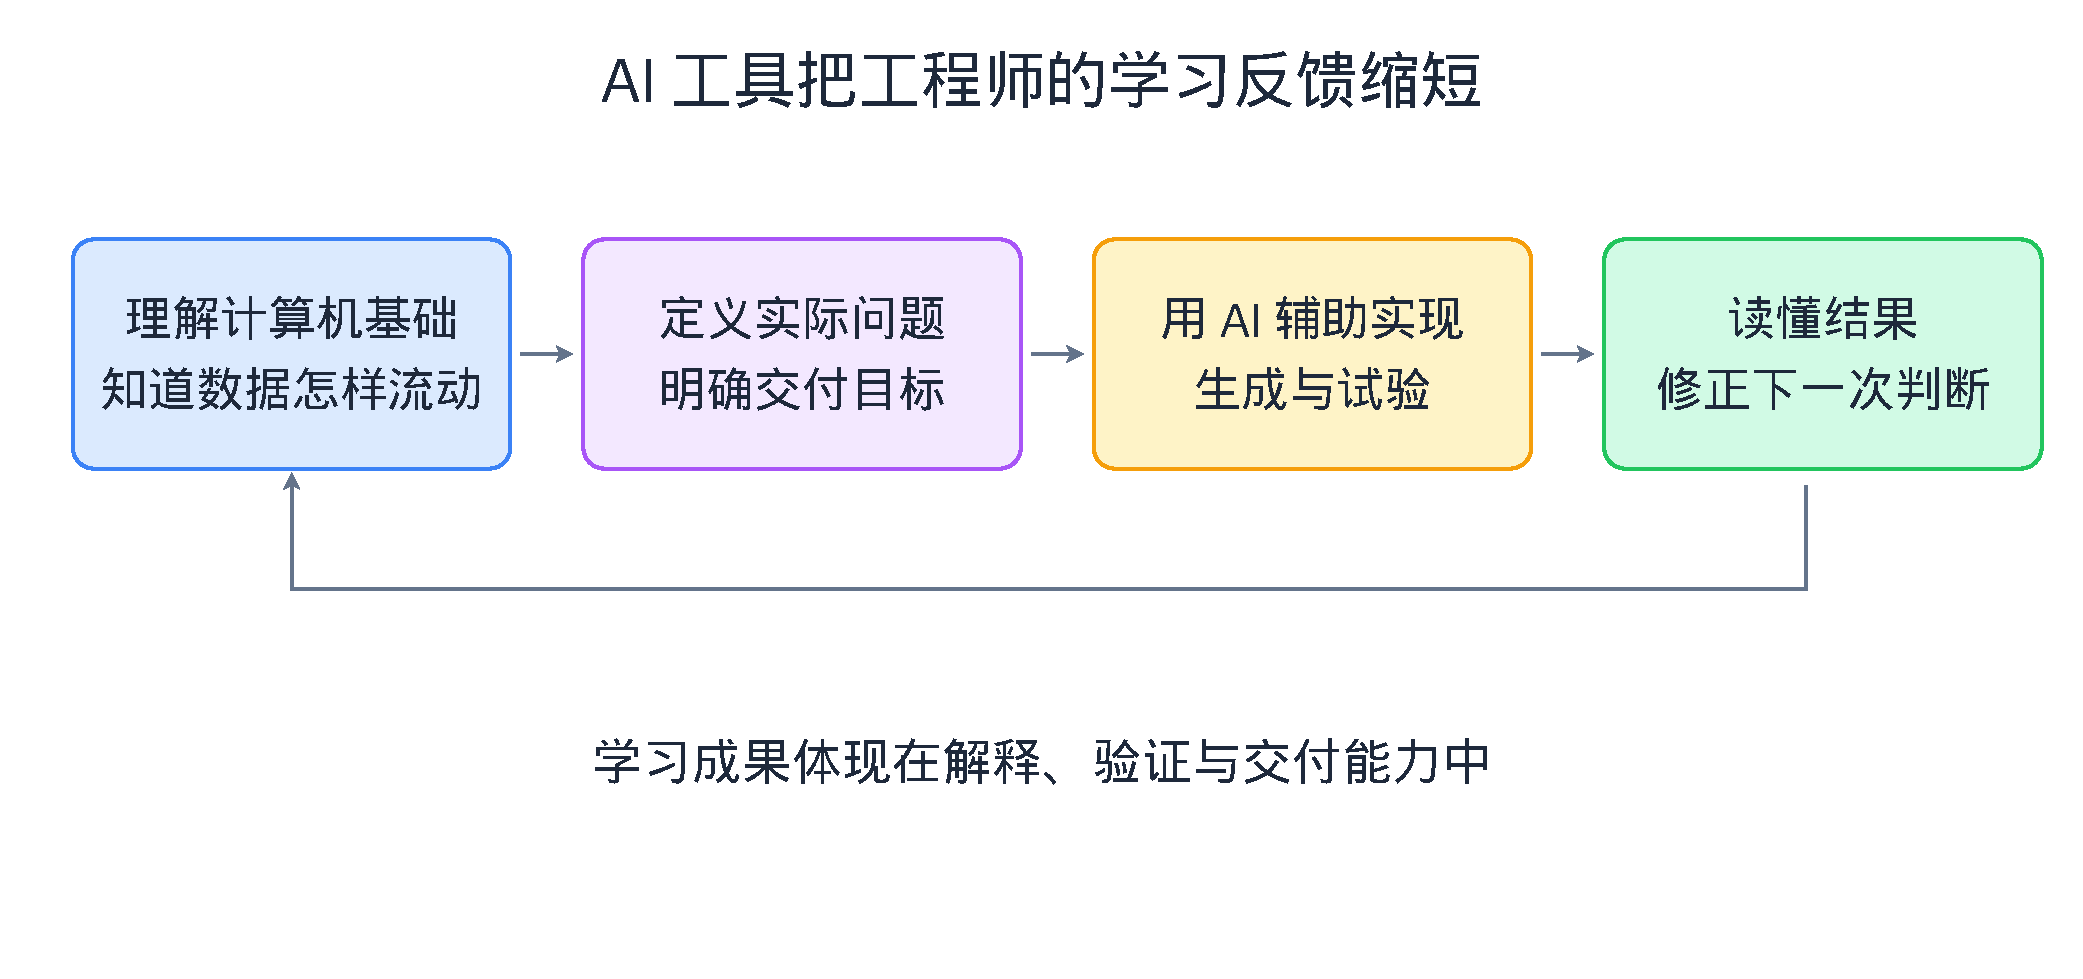
\includegraphics[width=\linewidth,height=.68\textheight,keepaspectratio]{assets/figure-08.pdf}
\caption{AI 工具把工程师的学习反馈缩短，依据节目口述整理（01:50:46–01:56:44）}
\end{figure}
\begin{knowledgebox}{读图：AI 时代的工程师：基础、工具与长期选择}
图 8 上方由左向右排列四个圆角矩形框，并通过箭头依次指向右侧：“理解计算机基础（知道数据怎样流动）”\ensuremath{\rightarrow}“定义实际问题（明确交付目标）”\ensuremath{\rightarrow}“用 AI 辅助实现（生成与试验）”\ensuremath{\rightarrow}“读懂结果（修正下一次判断）”。从最右侧“读懂结果”底部引出一条向左跨越全图的折返箭头，指回最左侧的“理解计算机基础”，形成持续迭代的闭环。图底部文字写道：“学习成果体现在解释、验证与交付能力中”。
\end{knowledgebox}
正如这一闭环所示，AI 工具缩短了从想法到试验的距离，但定义问题、读懂试验结果并修正判断，依然建立在对计算机底层数据流动与系统原理的理解之上。
\needspace{6\baselineskip}\subsection{本章小结}
本章作为全书尾声，顺着嘉宾的行业观察，对比了半导体公司与互联网云厂商的成本结构变化：随着云厂商的资本性支出（CAPEX）大幅投向 GPU 集群与电力基建，大模型在软件开发中正扮演类似“EDA 工具”的角色。面对这一趋势，嘉宾建议年轻工程师继续学好计算机底层原理，理解数据流动与商业模式，并在实践中利用 AI 工具缩短反馈闭环，培养系统权衡的判断品味（taste）与诀窍（know-how），努力具备架构师思维；同时他也探讨了生产力提升对普通从业者基本生活福利的支撑，以及未来社会可能出现的分工分化。
\needspace{8\baselineskip}\section{总结与延伸}
纵观肖志斌二十余年的技术轨迹，从单核多媒体指令扩展、众核片上数据流、处理器内嵌数据库加速单元，到专用 AI 推理芯片与数据中心级虚拟仿真，核心问题始终是如何消除计算、存储与通信之间的系统瓶颈。当先进制程微缩收益放缓、片上 SRAM 缩放受限、电力与晶圆扩产受制于物理周期时，单纯堆叠硬件已难以经济地降低词元成本。大模型推理在预填充与解码阶段的不同特征，既催生了 Groq、Cerebras、SambaNova 等数据流与混合存储路线，也凸显了通过算子、编译器、运行时调度与虚拟仿真挖掘现有硬件利用率的价值。

在尾声部分，肖志斌将大模型类比为软件工业的“EDA 工具”：随着云厂商资本性支出（CAPEX）比重上升，常规开发环节更多转为调用 AI 工具，而工程师的核心竞争力在于理解计算机底层数据流动、看懂业务与商业闭环，并在实践中积累系统权衡的判断品味（taste）与诀窍（know-how）。同时他也认为，生产力提升有望保障普通工具使用者的基本生活福利，但社会分工可能因此出现两极分化。

进一步学习与思考的问题：
\begin{enumerate}
\item 在给定模型结构、输入序列长度、批大小与数值精度的前提下，如何定量评估某项推理任务主要受限于计算吞吐、HBM 带宽还是跨节点互联？
\item 为什么开放指令集（如 RISC-V）或局部金属层修改方案，仍无法绕开微架构实现、商业 IP、EDA 协同与晶圆制造的工程成本？
\item 面对 MoE 动态专家路由与随机并发请求，静态系统仿真为何会产生偏差，又该如何设计低开销的实机剖析（profiling）数据回路来校准模型？
\end{enumerate}
\subsection{拓展阅读}
以下资料供回看节目、查阅术语与继续学习。
\begin{itemize}
\item 本期完整视频：\url{https://www.youtube.com/watch?v=gxeP0tAm8mc}
\item 官方完整逐字稿：\url{https://unclemoon.ai/blog/006-xiao-zhibin/transcript/}
\item 官方访谈文章：\url{https://unclemoon.ai/blog/006-xiao-zhibin/}
\item RISC-V International：开放指令集与生态：\url{https://riscv.org/about/}
\item NVIDIA CUDA Programming Guide：并行执行与存储层次：\url{https://docs.nvidia.com/cuda/cuda-programming-guide/index.html}
\end{itemize}
\end{document}
